\Chapter{Existing and Developed Software}{An Overview of \textsc{polsalt}, \textsc{iraf}, and \textsc{stops}} %% custom chapter command (defined in preamble)

This chapter contains an overview of \polsalt\ and the limitations faced during \polsalt\ wavelength calibrations (\autoref{sec:polsalt}), a brief overview of the \iraf\ tasks relevant for spectropolarimetric wavelength calibrations (\autoref{sec:iraf}), and an overview of \stops, the software developed to supplement the \polsalt\ reduction process (\autoref{sec:stops}). Finally, a discussion of the updated reduction process, an example of which may be found in \autoref{app:reduction}, is included (\autoref{sec:red_proc}).

% MARK: POLSALT
% http://salt-conference-2018.salt.ac.za/wp-content/uploads/2018/11/Groenewald.pdf
% https://saltworkshop2022.salt.ac.za/wp-content/uploads/2022/11/DG_polsalt_SALT_workshop_2022_finalversion.pdf
% https://github.com/saltastro/polsalt/wiki/Linear-Polarization-Reduction.--Beta-version#7-specpolfilterpy--compute-synthetic-filter-polarization-results-for-listed-filters
% https://github.com/saltastro/polsalt/wiki/
\section[\textsc{polsalt}]{\polsalt\ - \glsfmtlong{POLSALT}} \label{sec:polsalt}

\begin{figure}[t]
    \centering
    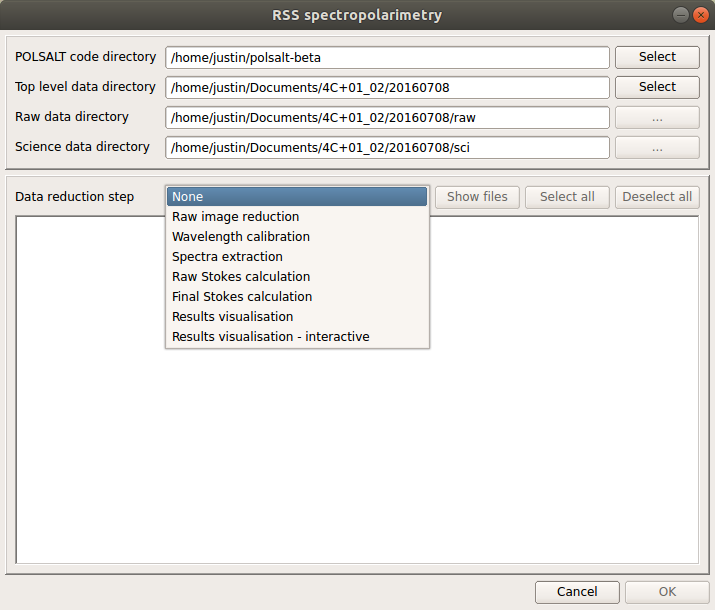
\includegraphics[width = 0.8\textwidth]{3_polsalt_GUI.png}
    \caption{The layout of the \polsalt\ \gls{GUI}, including the contents of the reduction steps accessible via the dropdown menu. Note that there is no trailing forward slash after the `Top level data directory'. Figure created from a local instance of the \polsalt\ \gls{GUI}.}
    \label{fig:polsalt_gui}
\end{figure}

The \polsalt\ (\glsxtrlong{POLSALT}) pipeline is the official reduction pipeline for spectropolarimetric data taken using the \gls{SALT} \gls{RSS}.%
\footnote{\polsalt\ is made freely available via the \polsalt\ GitHub repository, available at \url{https://github.com/saltastro/polsalt}. It is strongly advised to follow the wiki for installation instructions.}
The newest version of the software, aptly named the `beta version' (`version' 23 January 2020), was the version adapted in this study. It includes a \gls{GUI}, depicted in \autoref{fig:polsalt_gui}, which allows for limited interactivity during key steps in the reduction process.%
\footnote{Installation files and instructions for the `beta version' utilizing the \gls{GUI} are available at \url{http://www.saao.ac.za/~ejk/polsalt/code/} in a TAR GZIP file.}

The steps that make up the \polsalt\ reduction pipeline include raw image reductions, wavelength calibrations, background subtraction and spectral extraction, raw Stokes calculations, final Stokes calculations, and visualization of the results. Accurate reductions at each step are crucial for accurate results and are thus briefly discussed below. Further details for the reduction process may be found at the \href{https://github.com/saltastro/polsalt/wiki}{\polsalt\ GitHub wiki}.%
\footnote{The GitHub wiki for \polsalt\ is available at \url{https://github.com/saltastro/polsalt/wiki}.}

% MARK: Basic CCD reductions
\subsection{Raw Image Reductions} \label{subsec:pol_raw}

Raw image reductions are run via \textbf{imred.py} and apply the necessary basic reductions to the raw data before any calibrations are applied. These reductions include overscan subtractions, gain corrections, crosstalk corrections, and mosaicking as well as attaching the bad pixel maps and pixel variance information. Files with raw image reductions performed have ``mxgbp'' prepended to their names. As of February 2022, raw image reductions are automatically run for all RSS spectropolarimetric observations as part of the default SALT basic reduction pipeline that is run daily.

% MARK: Wavelength calibrations
\subsection{Wavelength Calibrations} \label{subsec:pol_wav}

Wavelength calibration and cosmic-ray rejection is performed via \textbf{specpolwavmap.py} and separately calibrates the $O$- and $E$-beams, based on the arc frames, and applies a simple cosmic-ray rejection for all science frames. This step is interactive and allows the user to individually fit wavelength calibration maps to each beam. The importance of an accurate correlation between both beams has been touched on previously (\autoref{subsec:specpol_cal}) and will be further discussed in \autoref{subsec:polsalt_limits}. The wavelength calibrated results are saved as an additional \gls{WAV} wavelength extension to each science FITS file, which are prefixed with a ``w'', and the $O$- and $E$-beams of the extensions are split into their own sub-extensions.

% MARK: Background subtraction and spectral extraction
\subsection{Spectral Extraction} \label{subsec:pol_spec}

\begin{figure}[t]
    \centering
    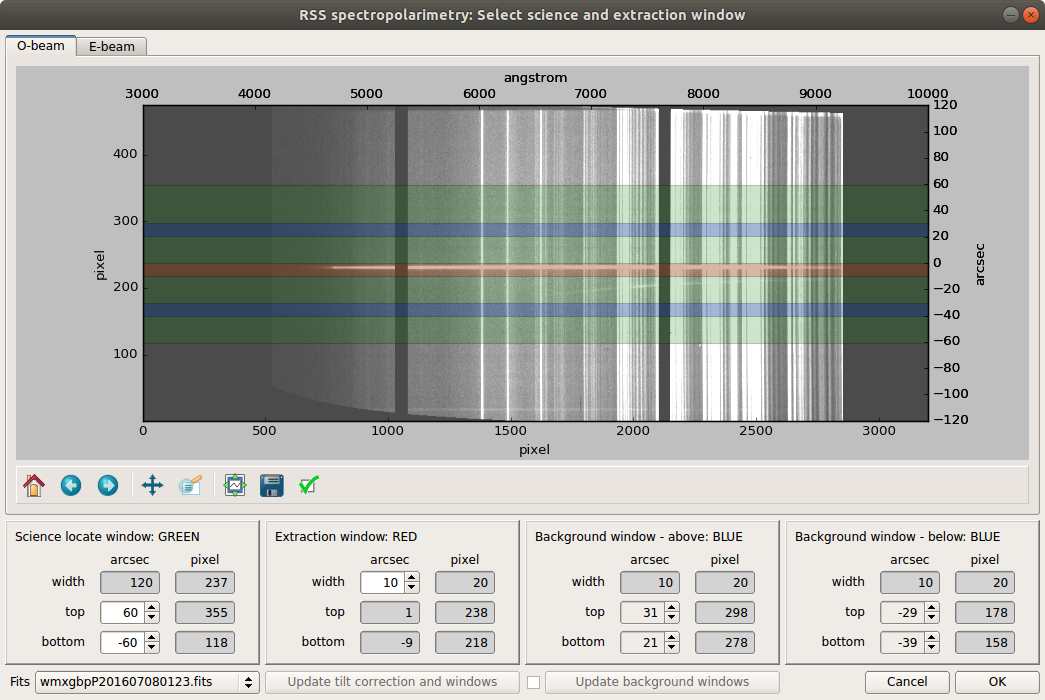
\includegraphics[width = 0.8\textwidth]{3_polsalt_tilt.png}
    \caption{The layout of the interactive \polsalt\ \texttt{spectra extraction} \gls{GUI} after selecting the `update tilt correction and windows' button along the bottom border of the window. Figure created from a local instance of the \polsalt\ \gls{GUI}.}
    \label{fig:polsalt_gui_spec}
\end{figure}

Background subtraction and spectral extraction is run via \textbf{spec\-pol\-extract\_dev.py} which corrects for the beam-splitter distortion and tilt, performs sky subtraction, and extracts a one dimensional wavelength dependent spectrum for each beam sub-extension. This step is interactive with \autoref{fig:polsalt_gui_spec} showing the interactive window used for spectral extraction.
The user, using the brightest trace in the image as a reference, defines regions which span the wavelength axis which define the background and trace regions for the sky subtraction and spectral extraction. Files with background and geometric corrections applied are saved with ``c'' prepended to their names and files which contain the extracted one dimensional spectrum have ``e'' further prepended to their names.

% MARK: Raw Stokes calculations
\subsection{Raw Stokes Calculations} \label{subsec:pol_rstokes}

The raw Stokes calculations are performed via \textbf{specpolraw\-stokes\_dev.py} and identify waveplate pairs for which the intensity, $I$, and a `raw Stokes' signal, $S$, are calculated as:
\begin{align} \label{eq:polsalt_rawstokes}
    I &= \frac{1}{2} (O_{1} + O_{2} + E_{1} + E_{2})\,,\ \text{and}\\
    S &= \frac{1}{2} \left[ \left( \frac{O_{1} - O_{2}}{O_{1} + O_{2}} \right) - \left( \frac{E_{1} - E_{2}}{E_{1} + E_{2}} \right) \right]\,.
\end{align}
The raw Stokes signal is calculated as the normalized difference of the $O$- and $E$-beams, for a waveplate pair, taken perpendicular to one another. The created files contain the raw Stokes information and use a very specific naming style; most notably the indexes of the related waveplate pairs, from \autoref{table:RSS_specpol_patterns}, are included in the file names.

% MARK: Final Stokes calculations
\subsection{Final Stokes Calculations} \label{subsec:pol_fstokes}

The Final Stokes calculations are performed via \textbf{specpolfinalstokes.py} and, using the waveplate pattern along with the raw Stokes signals, calibrates for the polarimetric zero-point and waveplate efficiency, and calculates the final Stokes parameters. Before the final Stokes calculations are performed, and if a sufficient number of redundant exposures were taken, the raw Stokes signals are culled to eliminate outlier signals which may arise from, for example, temporary atmospheric conditions affecting the signal. The culling is performed by comparing observation cycles against one another, comparing the deviation of the signal means which estimate the baseline systematic polarization fluctuations (due to imperfections in repeatability), and performing a $\chi^2$ analysis to eliminate any statistical outliers.

% MARK: Visualization
\subsection{Visualization} \label{subsec:pol_viz}

\begin{figure}[t]
    \centering
    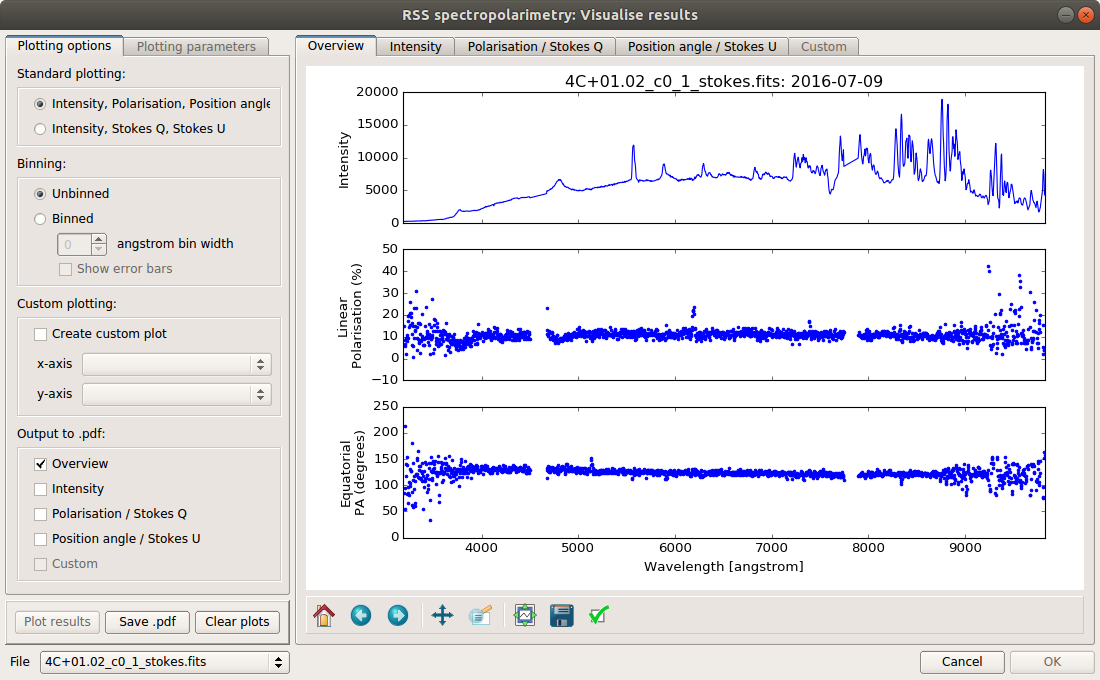
\includegraphics[width = 0.8\textwidth]{3_polsalt_viz.png}
    \caption{The layout of the interactive \polsalt\ \texttt{visualization} \gls{GUI} after selecting the `Plot results' button along the bottom border of the window. Figure created from a local instance of the \polsalt\ \gls{GUI}.}
    \label{fig:polsalt_gui_vis}
\end{figure}

Plotting the results of the spectropolarimetric reduction process is done using \textbf{specpol\-view.py}, which generates a plot of the Intensity, Linear Polarization ($\%$), and Equatorial Polarization Angle ($\degr$) against a shared wavelength axis, as seen in \autoref{fig:polsalt_plot}. This step is interactive allowing the user control over various options, such as the wavelength range, binning, etc., with the \gls{GUI} shown in \autoref{fig:polsalt_gui_vis}.

\begin{figure}[t]
    \centering
    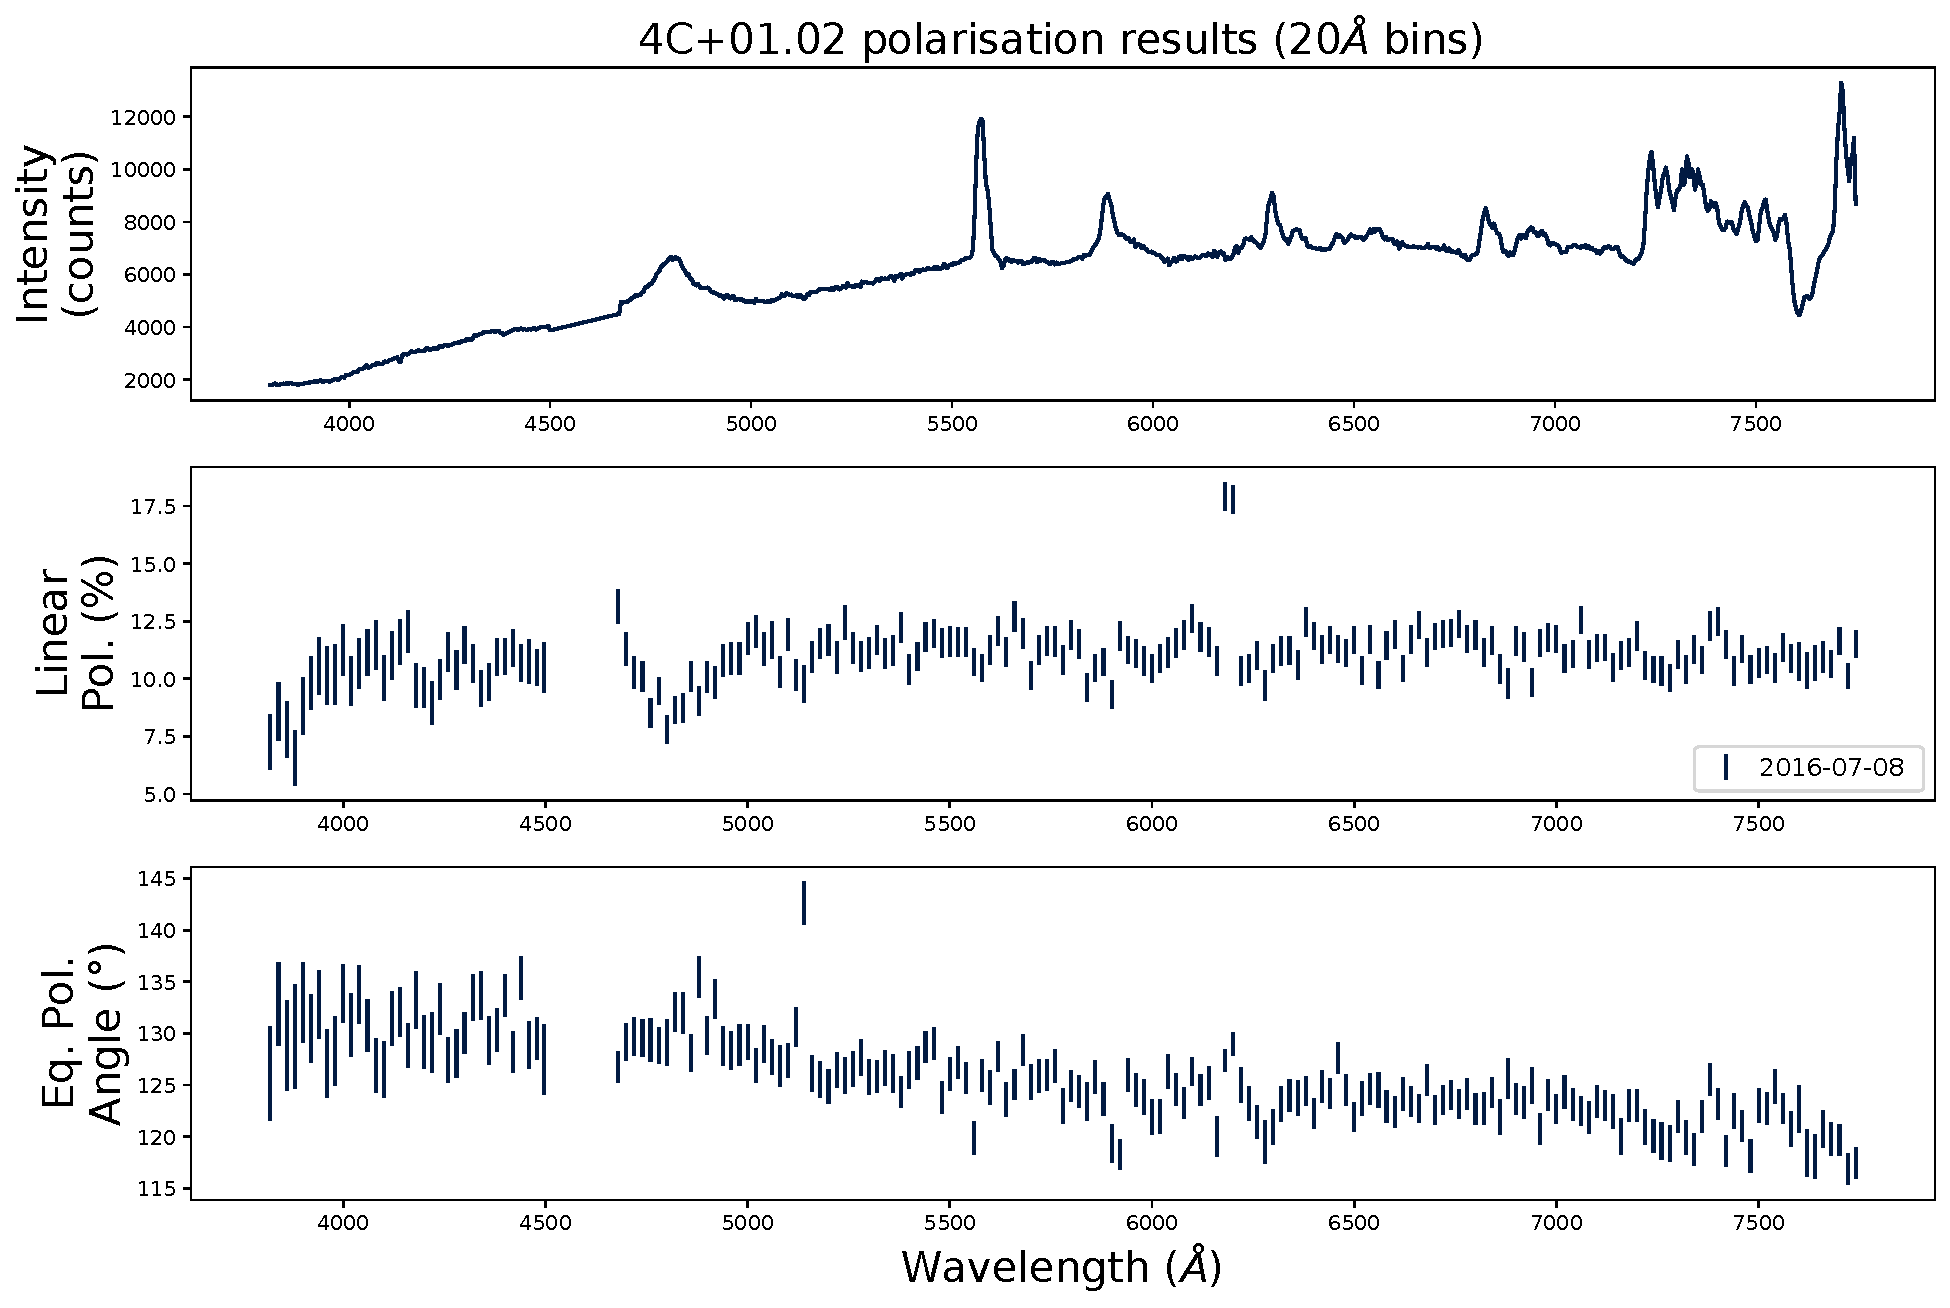
\includegraphics[width = 0.8\textwidth]{3_polsalt_plot.pdf}
    \caption{A typical plot resulting from the reduction process. Figure adapted from \citep{cooper_HEASA2022}.}
    \label{fig:polsalt_plot}
\end{figure}

% MARK: Post-processing analysis
\subsection{Post-Processing Analysis}

Generally, the plot of the spectropolarimetric results is the stopping point for most reduction procedures as it contains or creates the desired results. However, additional tools exist which may be used after the polarization reductions, and which are not represented in the \gls{GUI}, namely, flux calibration and synthetic filtering.

\pagebreak

Flux-calibrations are performed via \textbf{specpolflux.py} and are only intended for shape corrections of the spectrum. Additionally, a flux database file must exist for the observed standard and must be included in the working science directory.
% MARK: TODO: Flux Calibrations - errors in GUI - make 100\% sure about division error and notify Dani\'el

Synthetic filtering is calculated via \textbf{specpolfilter.py} and computes the synthetically filtered polarization results.
Any wavelength dependent throughput filter curve may be synthesized when defined by the user, but a few pre-defined filter curves are available, namely: the \glspl{SALTICAM} \gls{U}, \gls{B}, \gls{V}, \gls{R}, and \gls{I} Johnson-Cousins filter curves.

% MARK: Need for POLSALT
\subsection{\textsc{polsalt} Limitations and the Need for Supplementary Tools} \label{subsec:polsalt_limits}

% Why
The creation of supplementary tools for \polsalt\ spectropolarimetric reductions stemmed from the limitations of the wavelength calibration process and a need to compare wavelength solutions across the perpendicular $O$ and $E$ polarization beams. The process of calibrating wavelength solutions using the \polsalt\ pipeline is time-consuming for the average user, and often results in unexpected program crashes when receiving erroneous inputs or key presses. Due to the time-consuming process of recalibrating the wavelength solutions it is not feasible to perform the wavelength calibrations time and time again for anything larger than a handful of observations. This is particularly true for observations performed with the \gls{SALT} PG$0300$ grating as the sparse spectral features of the \gls{Ar} arc lamp are not handled well by the \polsalt\ pipeline.

% PG0300 reasoning
Since PG$0300$ provided the widest wavelength range and highest throughput, it was almost exclusively used for observations of flaring blazars, resulting in a large backlog of unanalyzed data. The only arc available for the PG$0300$ grating with a close enough articulation and grating angle ($\sim 10.68\degr$ and $\sim 5.38\degr$, respectively), was the \gls{Ar} arc lamp which displays sparse spectral features with large gaps over the wavelength range at these grating and articulation angles (\autoref{fig:ar_arc_salt}). This often led the \polsalt\ pipeline to create inconsistent wavelength solutions, or to fail to create a wavelength solution altogether, since minor deviations of identified spectral features resulted in large deviations in regions with no spectral features. To only further compound the difficulty of the wavelength calibrations, the spectrum of the \gls{Ar} arc lamp contains a partial overlap of a higher order at longer wavelengths (\autoref{subsubsec:diff_grat}, \autoref{eq:grating_equation}).

% How
The chosen solution to overcome the limitations of the wavelength calibration process was to use a well established wavelength calibration software which allowed for rapid recalibrations and provided a familiar interface. \iraf\ provides this familiar environment and reliability, in part thanks to its \href{https://github.com/iraf-community/iraf}{continued community development}.

Unfortunately, \iraf\ is unable to natively parse the data structure implemented by \polsalt\ `as is' and so the files must be restructured. This restructuring works both ways as once the \iraf\ reductions are complete the data structure must be restructured to match that of the \polsalt\ \texttt{wavelength calibration} output such that the reduction process may be completed in \polsalt.

\begin{figure}[t]
    \centering
    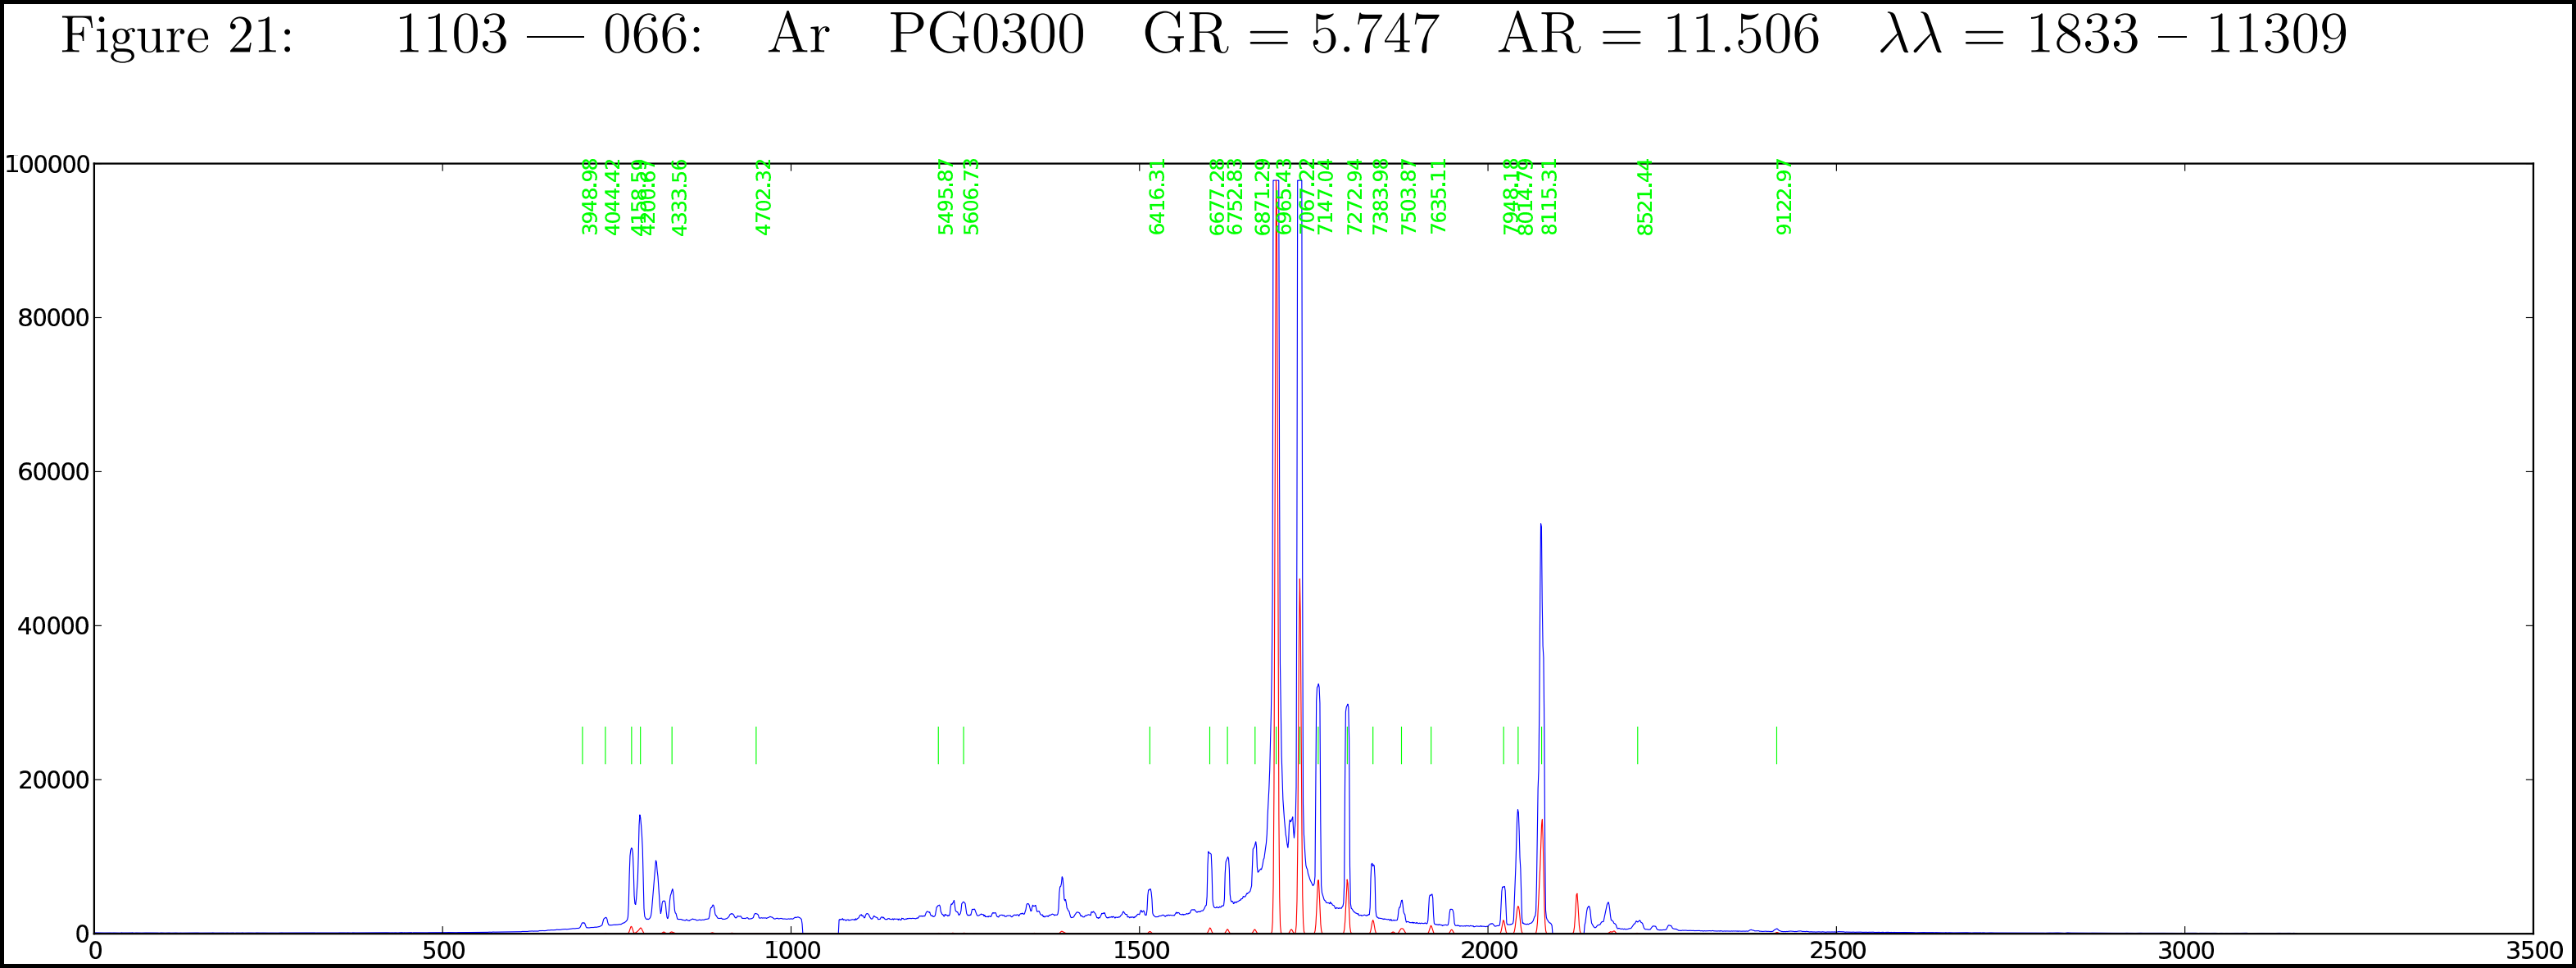
\includegraphics[width = 0.98\textwidth]{3_arc_spectrum.png}
    \caption{One of many \gls{Ar} arc lamp spectra as provided by \gls{SALT} for line identification. Plot adapted from \gls{SALT}'s published Longslit Line Atlases (as of 2024), resized to fit within the document margins but otherwise unchanged.\protect\footnotemark}
    \label{fig:ar_arc_salt}
\end{figure}
\footnotetext{\protect\href{https://pysalt.salt.ac.za/lineatlas/plot_line_argon_lores.pdf}{The `low resolution' Ar plot} sourced from \protect\url{https://astronomers.salt.ac.za/data/salt-longslit-line-atlas/}}

% MARK: IRAF
\section[\textsc{iraf}]{\iraf\ - \glsfmtlong{IRAF}} \label{sec:iraf}

% What is IRAF and why necessary
The \iraf\ (\glsxtrlong{IRAF}) software is a collection of software designed specifically for the reduction and analysis of astronomical images and spectra \citep{iraf:1986, iraf:1993}. The software consists of many tasks which perform specific operations and which are grouped into relevant packages. Only a brief overview of the tasks will be provided here. Help documentation for any of the \iraf\ tasks may be found online or through the \iraf\ \gls{CLI} through the \texttt{?} or \texttt{:.help} `cursor commands' when running interactive tasks, with more specific help documentation provided in the relevant section.%
\footnote{Online help for \iraf\ is available at \url{https://iraf.net/irafdocs/}}

Useful \iraf\ tasks that deserve a brief mention are: the \texttt{mkscript} task in the \texttt{system} package which allows a user to create and save a task along with the defined parameters as a file which can later be called as a script,%
\footnote{Help documentation for the \texttt{mkscript} task may be found at \url{https://astro.uni-bonn.de/~sysstw/lfa_html/iraf/system.mkscript.html}.}
the \texttt{implot} task in the \texttt{plot} package which allows the rows or columns of an image to be interactively displayed,%
\footnote{Help documentation for the \texttt{implot} task may be found at \url{https://astro.uni-bonn.de/~sysstw/lfa_html/iraf/plot.implot.html}.}
and the \texttt{eparam} task in the \texttt{language} package which allows the parameters of a task to be edited within the \iraf\ \gls{CLI}.%
\footnote{Help documentation for the \texttt{eparam} task may be found at \url{https://astro.uni-bonn.de/~sysstw/lfa_html/iraf/language.eparam.html}.}

For the wavelength calibration of \gls{SALT} spectropolarimetric data, the relevant tasks are the \texttt{identify} and \texttt{reidentify} tasks located in the \texttt{noao.onedspec} package, and the \texttt{fitcoords} and the (optional) \texttt{transform} tasks located under the \texttt{noao.twodspec.long\-slit} package. These tasks produce a two-dimensional wavelength solution which must be obtained separately for the $O$- and $E$-beam.

% MARK: Identify
\subsection{Identify} \label{subsec:iraf_identify}

The \texttt{identify} task is used to interactively determine a one-dimensional wavelength function across a chosen row of an arc exposure by identifying features in the spectrum with known wavelengths.%
\footnote{Help documentation for the \texttt{identify} task may be found at \url{https://astro.uni-bonn.de/~sysstw/lfa_html/iraf/noao.onedspec.identify.html}.}
The task creates the first approximation of the wavelength solution (see \autoref{fig:iraf_id_plot}) as well as a local database in which the solution is saved (see \autoref{lst:iraf_id_db}). The initial solution is built on in subsequent tasks, and it is, therefore, imperative that the initial solution is well-fit to minimize errors further along the calibration process.

% RMS
The execution of \texttt{identify} consists of identifying known features spanning the entire wavelength range and then removing any features which negatively impact the wavelength solution. A balance must be found between the number of identified features, the parameters of the fit, and the deviation of the fit from the known features.

\begin{lstlisting}[
    float,
    language=bash,
    style=IRAF_DB,
    caption={An example of the \texttt{identify} database contents.\protect\footnotemark},
    label=lst:iraf_id_db]
# Thu 15:19:16 13-May-2021
begin	identify arcO0057[*,237]
    id	arcO0057
    task	identify
    image	arcO0057[*,237]
    units	Angstroms
    features	35
              53.61 5944.74989   5944.834  13.0 1 1 15257
             140.19 6029.9793    6029.997  13.0 1 1  4652
             185.30 6074.34644   6074.338  13.0 1 1 13396
             207.49 6096.15873   6096.161  13.0 1 1 21700
             255.23 6143.0493    6143.063  13.0 1 1 33330
             276.13 6163.56995   6163.594  13.0 1 1 11344
             330.89 6217.29293   6217.281  13.0 1 1 13705
             381.10 6266.51524   6266.495  13.0 1 1 21747
             420.21 6304.8113    6304.789  13.0 1 1 10226
             450.49 6334.45415   6334.428  13.0 1 1 36235
             500.18 6383.04826   6382.991  13.0 1 1 35824
             519.85 6402.26802   6402.248  13.0 1 1 70163
             626.70 6506.56147   6506.528  13.0 1 1 46165
             653.73 6532.91083   6532.882  13.0 1 1 21413
             721.60 6598.98642   6598.953  13.0 1 1 26396
             803.21 6678.31069   6678.277  13.0 1 1 51338
             843.15 6717.0732    6717.043  13.0 1 1 36780
            1099.95 6965.36335   6965.431  13.0 1 1  5618.4  ar
            1169.57 7032.38598   7032.413  13.0 1 1 100000
            1317.05 7173.89814   7173.938  13.0 1 1  5000    decrease
            1391.52 7245.11148   7245.167  13.0 1 1 73545
            1537.20 7383.93022   7383.981  13.0 1 1  5557.5  ar
            1595.02 7438.83545   7438.898  13.0 1 1 15000    decrease
            1663.64 7503.86263   7503.869  13.0 1 1 30000    ar; increase
            1697.46 7535.84584   7535.774  13.0 1 1  8000    increase
            1802.64 7635.07335   7635.106  13.0 1 1 20000    ar; decrease
            2209.19 8014.79559   8014.786  13.0 1 1  3000    ar; decrease
            2604.58 8377.66137   8377.607  13.0 1 1 14543
            2734.54 8495.41423   8495.359  13.0 1 1  8765
            2763.48 8521.52355   8521.442  13.0 1 1  4537.5  ar
            2840.92 8591.20799   8591.258  13.0 1 1  2000    decrease
            2889.39 8634.67334   8634.647  13.0 1 1  3059
            2911.42 8654.39264   8654.383  13.0 1 1  3000    decrease
            2926.56 8667.93501   8667.944  13.0 1 1   702.5  ar
            3135.72 8853.77575   8853.867  13.0 1 1  1820
    function legendre
    order 4
    sample *
    naverage 1
    niterate 0
    low_reject 3.
    high_reject 3.
    grow 0.
    coefficients	8
        2.
        4.
        53.60757446289061
        3135.715576171875
        7425.420339270724
        1457.513831286474
        -26.15751926622308
        -3.000903509842187

\end{lstlisting}
\footnotetext{See also \url{https://iraf.net/irafdocs/formats/identify.php} for an explanation of the database contents.}

\begin{figure}
    \centering
    \begin{subfigure}[b]{0.49\textwidth}
        \centering
        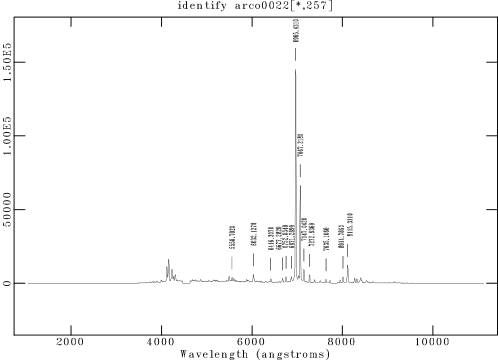
\includegraphics[width=\textwidth]{3_id.png}
        \caption{Identified features.}
    \end{subfigure}
    \hfill
    \begin{subfigure}[b]{0.49\textwidth}
        \centering
        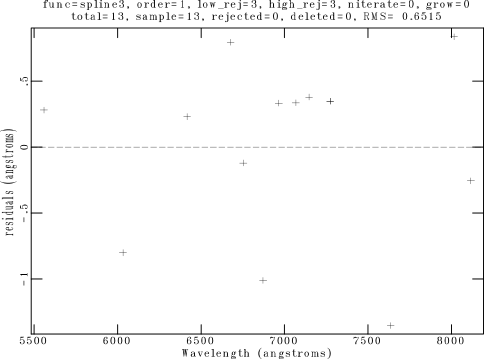
\includegraphics[width=\textwidth]{3_id_resids.png}
        \caption{\gls{RMS} of the identified features.}
    \end{subfigure}
    \caption{A plot and the \gls{RMS} of the identified features found using the \iraf\ \texttt{identify} task. Figures created using the \iraf\ \texttt{identify} task.}
    \label{fig:iraf_id_plot}
\end{figure}

% MARK: Reidentify
\subsection{Reidentify} \label{subsec:iraf_reidentify}

The \texttt{reidentify} task is used to run the \texttt{identify} task autonomously and repeatedly across the entirety of the arc frame at defined (row) intervals.%
\footnote{Help documentation for the \texttt{reidentify} task may be found at \url{https://astro.uni-bonn.de/~sysstw/lfa_html/iraf/noao.onedspec.reidentify.html}.}
The task uses the one-dimensional wavelength solution stored in the database created by the initial \texttt{identify} call and refits the positions of the relevant spectral features. The task may fail based on a number of conditions, most common of which is the loss of features as the task moves further from the row at which the user manually ran \texttt{identify}.

\pagebreak

When running \texttt{reidentify} non-interactively, it is recommended to set the \texttt{verbose} parameter to `\texttt{yes}' as this will provide immediate confirmation if the task quit early. Regardless of whether the task quit successfully, the newly defined wavelength solutions are appended to the local database following the \texttt{identify} task database format, an example of which is given in \autoref{lst:iraf_id_db}.

% MARK: Fitcoords
\subsection{Fitcoords} \label{subsec:iraf_fitcoords}

The \texttt{fitcoords} task is used to find a two-dimensional surface function from the one-dimensional wavelength solutions found for specific rows in the previous steps.%
\footnote{Help documentation for the \texttt{fitcoords} task may be found at \url{https://astro.uni-bonn.de/~sysstw/lfa_html/iraf/noao.twodspec.longslit.fitcoords.html}.}
The usage of \texttt{fitcoords} is similar to that of \texttt{identify} and consists of examining the distribution of identified points and eliminating any points that \texttt{reidentify} may have misidentified (see \autoref{fig:iraf_fc_plot}).

By eliminating outliers with bad residuals and modifying the two-dimensional surface function's type and degree, the overall error of the fit is decreased, aligning more closely to what the `true' wavelength solution is.
This surface function is the final two-dimensional wavelength solution for each two-dimensional spectrum. It is saved using the \texttt{fitcoords} database format, an example of which is given in \autoref{lst:iraf_fc_db}, as the list of parameters and function coefficients required to recreate the closest two-dimensional model. The \iraf\ wavelength solution is used by the \stops\ \texttt{join} method to create the \gls{WAV} extension required by \polsalt, further described in \autoref{subsec:stops_join}.

\begin{lstlisting}[
    float,
    language=bash,
    style=IRAF_DB,
    caption={An example of the \texttt{fitcoords} database contents.\protect\footnotemark},
    label=lst:iraf_fc_db]
# Thu 15:26:55 13-May-2021
begin	arcO0057
	task	fitcoords
	axis	1
	units	angstroms
	surface	33
		1.
		5.
		5.
		1.
		1.
		3199.
		1.
		474.
		7419.096745914063
		1510.03933621895
		-21.10886852752348
		-2.079553916887794
		0.06772631420528228
		0.7720164913117386
		-1.506773900054024
		0.1341878190232142
		-0.01659697703758917
		0.0251087019569153
		-3.318493303995171
		-0.3612632489821799
		0.003270665801371641
		-0.0157962041414068
		-0.003073690871589242
		0.007533453962924031
		0.02839687304474069
		-0.003233465769521899
		0.00174111456659807
		0.00645177595090841
		0.0105080093855621
		-0.01157827440314294
		-0.007789479002470706
		-0.006562085282926231
		-0.002321476801926803

\end{lstlisting}
\footnotetext{See also \url{https://iraf.net/irafdocs/formats/fitcoords.php} for an explanation of the database contents.}

\begin{figure}
    \centering
    \begin{subfigure}[b]{0.49\textwidth}
        \centering
        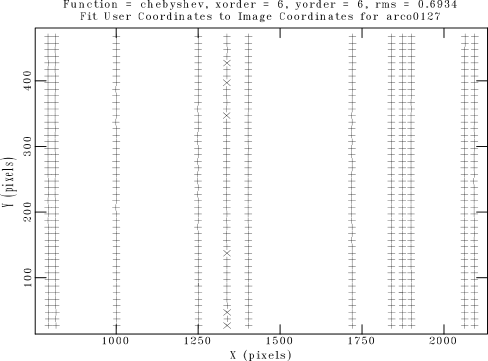
\includegraphics[width=\textwidth]{3_fc.png}
        \caption{Features identified across an exposure.}
    \end{subfigure}
    \hfill
    \begin{subfigure}[b]{0.49\textwidth}
        \centering
        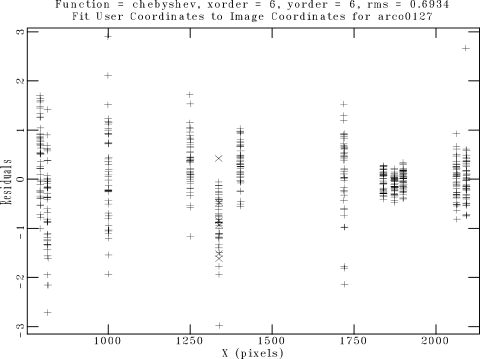
\includegraphics[width=\textwidth]{3_fc_resids.png}
        \caption{\gls{RMS} of the identified features.}
    \end{subfigure}
    \caption{A plot and the \gls{RMS} of the features identified across the exposure using the \iraf\ \texttt{fitcoords} task. Figures created using the \iraf\ \texttt{fitcoords} task.}
    \label{fig:iraf_fc_plot}
\end{figure}

% MARK: Transform
\subsection{Transform} \label{subsec:iraf_transform}

The \texttt{transform} task is the optional final step in the \iraf\ wavelength calibration process.%
\footnote{Help documentation for the \texttt{transform} task may be found at \url{https://astro.uni-bonn.de/~sysstw/lfa_html/iraf/noao.twodspec.longslit.transform.html}.}
Simply put, \texttt{transform} converts the ($x_p$, $y_p$) pixel units of an exposure to ($\lambda$, $y_p$) wavelength units which allows for an immediate check of whether the wavelength solution is consistent across the frame. Any general error in the wavelength solution may be spotted in the transformed images; ranging from minor errors, such as the arc lines or sky lines not being purely vertical across the frame, to more major errors, such as an incorrect wavelength solution skewing the exposure beyond recognition.

For example, \autoref{subfig:trans_O} shows a good fit to the wavelength solution, as after transformation all the sky lines run exactly vertical. \autoref{subfig:trans_E}, on the other hand, shows a seemingly good fit, but closer inspection reveals that the sky lines (especially towards the right of the frame) deviate from the vertical, indicating a poor fit to the wavelength solution.

\begin{figure}[t]
    \centering
    \begin{subfigure}[b]{1.0 \textwidth}
        \centering
        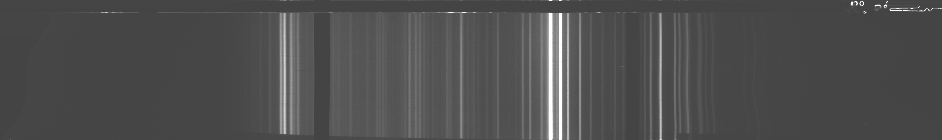
\includegraphics[width=\textwidth]{3_tarcO.pdf}
        \caption{A poorly fit wavelength solution with a region of no exposure (top of frame).}
        \label{subfig:trans_O}
    \end{subfigure}
    \centering
    \begin{subfigure}[b]{1.0\textwidth}
        \centering
        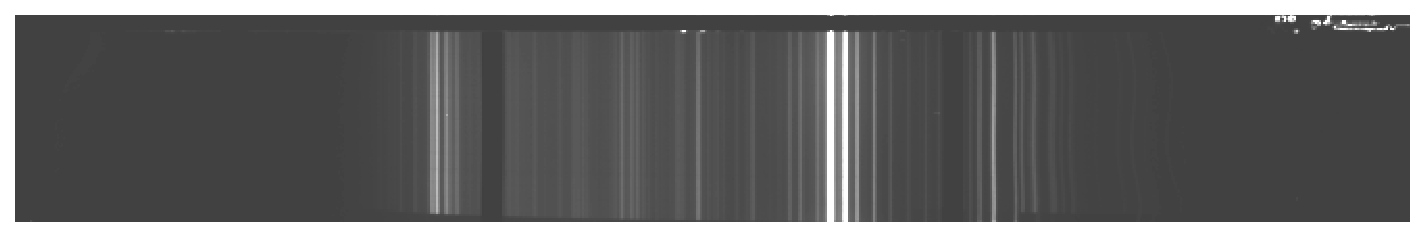
\includegraphics[width=\textwidth]{3_tarcE.pdf}
        \caption{A well-fit wavelength solution.}
        \label{subfig:trans_E}
    \end{subfigure}
    \caption{Examples of a poor fit (\subref{subfig:trans_O}) and well-fit (\subref{subfig:trans_E}) wavelength solution applied to the $O$- and $E$-beams of an arc image. The contrast of the figures were scaled to best capture any deviation of the arc lines. Figures created by the \iraf\ \texttt{transform} task.}
    \label{fig:iraf_trans_plot}
\end{figure}

% MARK: STOPS
\section[\textsc{stops}]{\stops\ - \textit{Supplementary Tools for \textsc{polsalt}\\Spectropolarimetry}} \label{sec:stops}

\glsxtrfull{STOPS} provides supplementary tools which convert the \polsalt\ and \iraf\ formats back and forth, allowing \iraf\ to be used for wavelength calibrations of \gls{SALT} spectropolarimetric data. It also provides additional tools to check the accuracy of the wavelength calibration.
\stops\ is written in, and requires, Python~$3$ ($3.11+$) to run, as well as \texttt{Astropy} ($6.0.0+$) \citep{astropy:2013, astropy:2018, astropy:2022}, \texttt{ccdproc} ($2.4.1+$) \citep{ccdproc}, \texttt{Matplotlib} ($3.5.2+$) \citep{matplotlib}, \texttt{NumPy} ($1.26.4+$) \citep{numpy}, and \texttt{SciPy} ($1.13.0+$) \citep{scipy}.

The parsing of \polsalt\ data into an \iraf\ usable format and the reformatting of the \iraf\ wavelength calibrated data back into a \polsalt\ usable format, referred to as \textit{splitting} and \textit{joining}, is performed by the \stops\ \texttt{split} and \texttt{join} methods, respectively.

Methods to verify the validity of the wavelength calibrations were also added to \stops. The \texttt{skyline} method checks the sky line wavelength ($x$) positions across the frame as well as the variation of the sky lines across the positional ($y$) axis of the frame. The \texttt{correlate} method checks the correlation of the $O$- and $E$-beams either within a given \gls{FITS} file or across multiple files (comparing only the $O$- and $E$-beams for each). With these two additional methods, a user is able to verify that the wavelength solutions do not conflict across the $O$- and $E$-beams and that no unexpected deviations are included in the wavelength solutions.

Help on the usage of \stops\ in a \gls{CLI} can be viewed by running:
\begin{lstlisting}[language=bash]
$ python ~/STOPS --help
# OR
$ python ~/STOPS [split|join|correlate|skylines] --help
\end{lstlisting}
{\parskip=0pt which} retrieves and prints the help documentation to the \gls{CLI} from \autoref{source:main} (in \autoref{app:code}), such as how to enable logging or increase the verbosity, or change default parameters of the various methods. Finally, help documentation for the specific \stops\ methods may be found within this section (\autoref{doc:split} to \ref{doc:corr}) or in \autoref{app:code}.

% MARK: Split
\subsection{Splitting} \label{subsec:stops_split}

\lstinputlisting[
    float,
    language=python,
    style=STOPS_docs,
    caption={The `docstring' for \textbf{split.py}},
    label=doc:split,
    linerange=split0-split1,
    gobble=4,
]{split.py}

% Why necessary
As mentioned previously, the format of the \gls{FITS} file created by \polsalt\ after basic \gls{CCD} reductions and the format expected by \iraf\ to be used for the wavelength calibrations are incompatible. Basic \polsalt\ \gls{CCD} reductions return \gls{FITS} files which contain a primary header along with extensions for the science, variance, and \gls{BPM} images. These extensions carry the image of the trace (see \autoref{fig:OE_split}), the variance of the image, and a map of the pixels to be masked out, split into sub-extensions for both polarimetry beams, respectively.

While \iraf\ is capable of dealing with multiple traces in an extension or lists of input files, it is not as capable when dealing with multiple wavelength solutions contained in a single extension (as expected by the \polsalt\ \texttt{wavelength calibration}) or extensions containing sub-extensions (as expected by the \polsalt\ \texttt{spectral extraction}). To simplify the \iraf\ reduction procedure it was decided to separate the perpendicular polarization beams into their own files.

% What it does -> Primary focus
The files with \polsalt\ pre-reductions applied, namely \gls{FITS} files with an `mxgbp' prefix (\autoref{sec:polsalt}), are used as the starting point for the supplementary tool's \texttt{split} method. Running \texttt{split} finds all the \gls{FITS} files for wavelength calibration within the working directory, creates two empty \gls{HDU} structures for each \gls{FITS} file (i.e. for both the $O$- and $E$-beam), and appends all header and science data necessary for wavelength calibration to the relevant \gls{HDU} structure. Otherwise, defaults, such as which row to split the image along to separate the beams, were kept as close to the \polsalt\ pipeline as possible.

\begin{figure}[t]
    \centering
    \begin{subfigure}[b]{1.0 \textwidth}
        \centering
        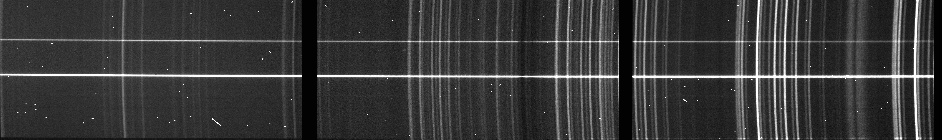
\includegraphics[width=\textwidth]{3_splitO.pdf}
        \caption{The $O$-beam region of the \gls{FITS} file.}
        \label{subfig:split_O}
    \end{subfigure}
    \centering
    \begin{subfigure}[b]{1.0\textwidth}
        \centering
        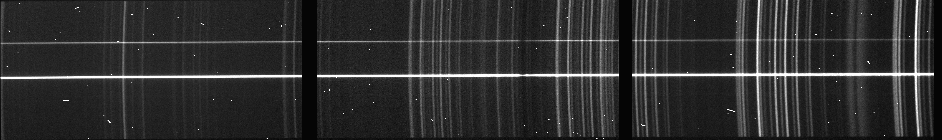
\includegraphics[width=\textwidth]{3_splitE.pdf}
        \caption{The $E$-beam region of the \gls{FITS} file.}
        \label{subfig:split_E}
    \end{subfigure}
    \caption{The split $O$- (\subref{subfig:split_O}) and $E$-beams (\subref{subfig:split_E}) as handed to \iraf. Figure created from the \stops\ \texttt{split} method output.}
    \label{fig:OE_split}
\end{figure}

% Focus on minimizing changes and optimizing size
As the intent was always to parse the wavelength function back into \polsalt\ it was decided to keep these temporary \gls{FITS} files as small as possible by only including the header and \gls{SCI} science extension.
% This is especially necessary when considering the amount of exposures taken for long term studies. % for a single spectropolarimetric observation run, and how the number of observations increases
%
% Any changes from how polsalt would do it
To aid the scripting of the \iraf\ wavelength calibration process, the \texttt{split} method also performs row cropping to exclude \gls{CCD} regions which are not exposed to light, and creates files listing the split $O$- and $E$-beam \gls{FITS} files which may be passed to the \iraf\ task inputs. Row cropping was decided on as \iraf\ does not handle rows with no exposure well, specifically when it comes to the autonomous \texttt{reidentify} task.
The full \stops\ \texttt{split} class docstring is given in \autoref{doc:split}.

% MARK: Join
\subsection{Joining} \label{subsec:stops_join}

\lstinputlisting[
    float,
    language=python,
    style=STOPS_docs,
    caption={The `docstring' for \textbf{join.py}},
    label=doc:join,
    linerange=join0-join1,
    gobble=4,
]{join.py}

% Running \texttt{join} finds all the relevant \gls{FITS} and local \iraf\ database files, creates an empty \gls{HDU} structure for each pair of matching spectropolarimetric beams, copies over the extensions and their respective image and header information, appends a new \gls {WAV} extension and parses the database wavelength solutions into the \polsalt\ intensity-wavelength format, performs cosmic ray cleaning, and masks the \gls{BPM} to reflect the wavelength calibrated regions.
After the \iraf\ \texttt{fitcoords} task has been successfully run for both the $O$- and $E$-beams, the \stops\ \texttt{join} method is used to extract and parse the wavelength solution from the \iraf\ database, and to create the wavelength calibrated \gls{FITS} files required by the \polsalt\ pipeline. More specifically, the \texttt{join} method performs the following steps:

First, \texttt{join} parses the wavelength database file, described in \autoref{subsec:iraf_fitcoords}, for either a `Chebyshev' or `Legendre' solution, and calculates the wavelength at each ($x_{p}$, $y_{p}$) pixel position. This new image containing the corresponding wavelength values, seen in \autoref{fig:pol_wav_ext}, is appended to the wavelength calibrated \gls{FITS} file as the \gls{WAV} extension.
% and creates a function to convert a ($pixel$, $pixel$) position to a wavelength value. This is used to fill the pixels of the \gls{WAV} extension with their respective wavelength, as seen in \autoref{fig:pol_wav_ext}.

\pagebreak

% cosmic ray cleaning
Second, cosmic-ray cleaning is performed on the \gls{SCI} extension using the \texttt{ccdproc} implementation of the \texttt{lacosmic} Python package which implements the L.A. Cosmic algorithm, based on Laplacian edge detection. The read noise and gain parameters used for cosmic ray cleaning were chosen based on the properties of the \gls{RSS}, while the rest of the parameters were left as the default, following the publication and \href{http://www.astro.yale.edu/dokkum/lacosmic/pars.html}{suggestions}%
\footnote{Suggested parameters for the \texttt{lacosmic} algorithm may be found at \url{http://www.astro.yale.edu/dokkum/lacosmic/pars.html}.}
by the algorithm's creator, as well as the implementation of the algorithm in the python \texttt{ccdproc} package \citep{lacosmic,astroscrappy}. The chosen parameters work well for most cosmic rays, as can be seen when comparing \autoref{fig:OE_split} to \autoref{fig:polsalt_post_wav_cal}, but may be modified as needed.

% update headers
% copy data, double check shape change
Next, \texttt{join} updates the headers to be near-identical to those created by the \polsalt\ \texttt{wavelength calibration}, most notably updating the data shape, `CTYPE3', and data type, `BITPIX', keywords.
The only difference in the header is the  `NAXIS2' keyword, due to the cropping performed by \texttt{split}. The cropped region could be reintroduced but would be masked out and further discarded in the following \polsalt\ \texttt{spectra extraction} process, making it redundant.

\begin{figure}[t]
    \centering
    \begin{subfigure}[b]{1.0 \textwidth}
        \centering
        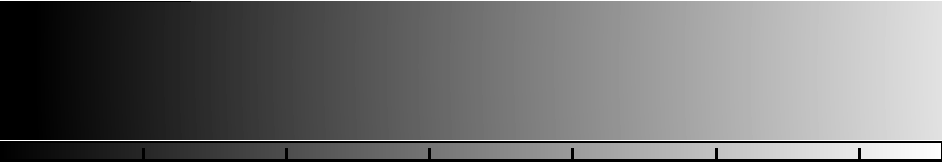
\includegraphics[width=\textwidth]{3_pol_wav_O.pdf}
        \caption{The $O$ polarimetric beam.}
        \label{subfig:pol_O}
    \end{subfigure}
    \centering
    \begin{subfigure}[b]{1.0\textwidth}
        \centering
        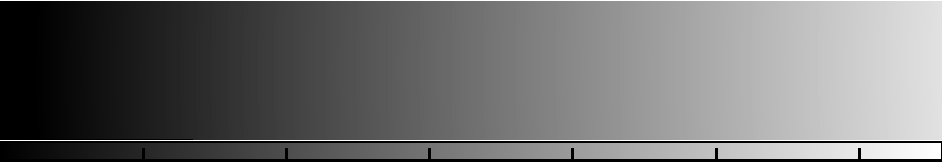
\includegraphics[width=\textwidth]{3_pol_wav_E.pdf}
        \caption{The $E$ polarimetric beam.}
        \label{subfig:pol_E}
    \end{subfigure}
    \caption{A representative \gls{WAV} extension of a \gls{FITS} file, for the $O$- (\subref{subfig:pol_O}) and $E$-beam (\subref{subfig:pol_E}), ready to be processed by the \polsalt\ pipeline. The color bars show the wavelength in \AA. Note that regions which fall outside the exposed region are masked by setting the corresponding pixel values of the wavelength and \gls{BPM} extensions to $0$. Figure created from the \stops\ \texttt{join} method output.}
    \label{fig:pol_wav_ext}
\end{figure}

% polsalt specific cropping (wav mask)
% mask wavelength using wollaston curve for polsalt `parsability'
% update BPM to reflect wavelength cropping
Finally, the \gls{WAV} extension is masked to remove any uncalibrated wavelength regions as well as masked for the skewing of the trace introduced by the wollaston element. The masking of the wollaston skewing is necessary since \polsalt\ introduces a wollaston correction in the \texttt{spectra extraction} process. The \gls{BPM} extension is masked to reflect the valid wavelength calibrated region, and the files are saved with the \polsalt\ wavelength calibrated `wmxgbp' prefix.
The full \stops\ \texttt{join} class docstring is given in \autoref{doc:join}.

\begin{figure}[t]
    \centering
    \begin{subfigure}[b]{1.0 \textwidth}
        \centering
        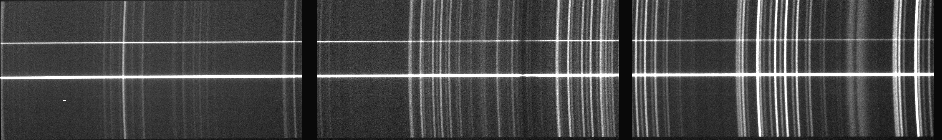
\includegraphics[width=\textwidth]{3_post_wav_cal_O.pdf}
        \caption{The $O$ polarimetric beam.}
        \label{subfig:post_wav_O}
    \end{subfigure}
    \centering
    \begin{subfigure}[b]{1.0\textwidth}
        \centering
        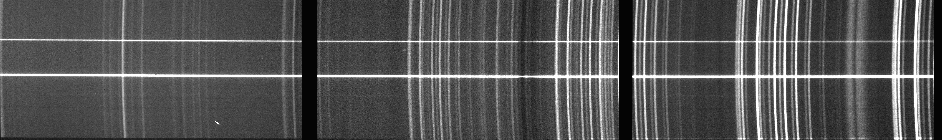
\includegraphics[width=\textwidth]{3_post_wav_cal_E.pdf}
        \caption{The $E$ polarimetric beam.}
        \label{subfig:post_wav_E}
    \end{subfigure}
    \caption{A representative \gls{SCI} extension of a \gls{FITS} file, for the $O$- (\subref{subfig:post_wav_O}) and $E$-beam (\subref{subfig:post_wav_E}), ready to be processed by the \polsalt\ pipeline. The observed intensity is displayed via the grayscale value at each pixel. Figure created from the \stops{join} method output.}
    \label{fig:polsalt_post_wav_cal}
\end{figure}
% Note the: chip gaps demarcated by regions of no exposure, traces which are regions of higher intensity spanning the horizontal axis, and sky lines which are the (slightly curved) regions of higher intensity strectching the vertical axis.

% MARK: Skyline
\subsection{Sky Line Checks} \label{subsec:stops_skyline}

\lstinputlisting[
    float,
    language=python,
    style=STOPS_docs,
    caption={The `docstring' for \textbf{skylines.py}},
    label=doc:skylines,
    linerange=sky0-sky1,
    gobble=4,
]{skylines.py}

\begin{figure}[t]
    \centering
    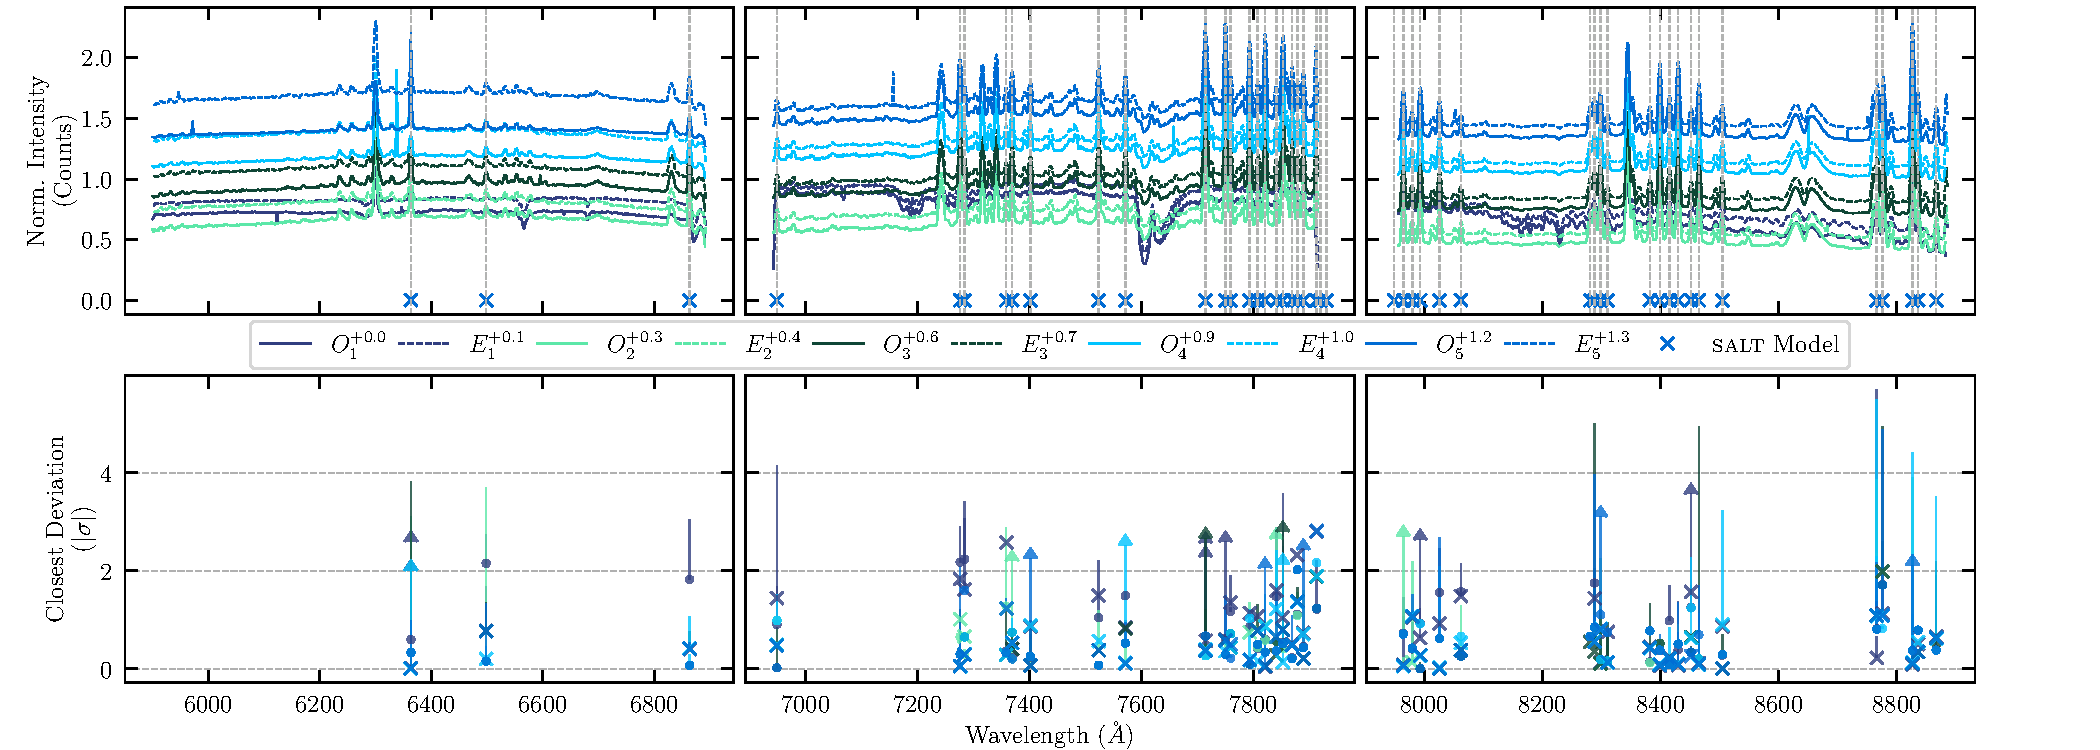
\includegraphics[width = 1.0\textwidth]{3_stops_skylines.pdf}
    \caption{An example of a well calibrated wavelength solution, specifically shown for science images. Figure created via the \stops\ \texttt{skyline} method.}
    \label{fig:stops_sky_eg}
\end{figure}
\begin{figure}[t]
    \centering
    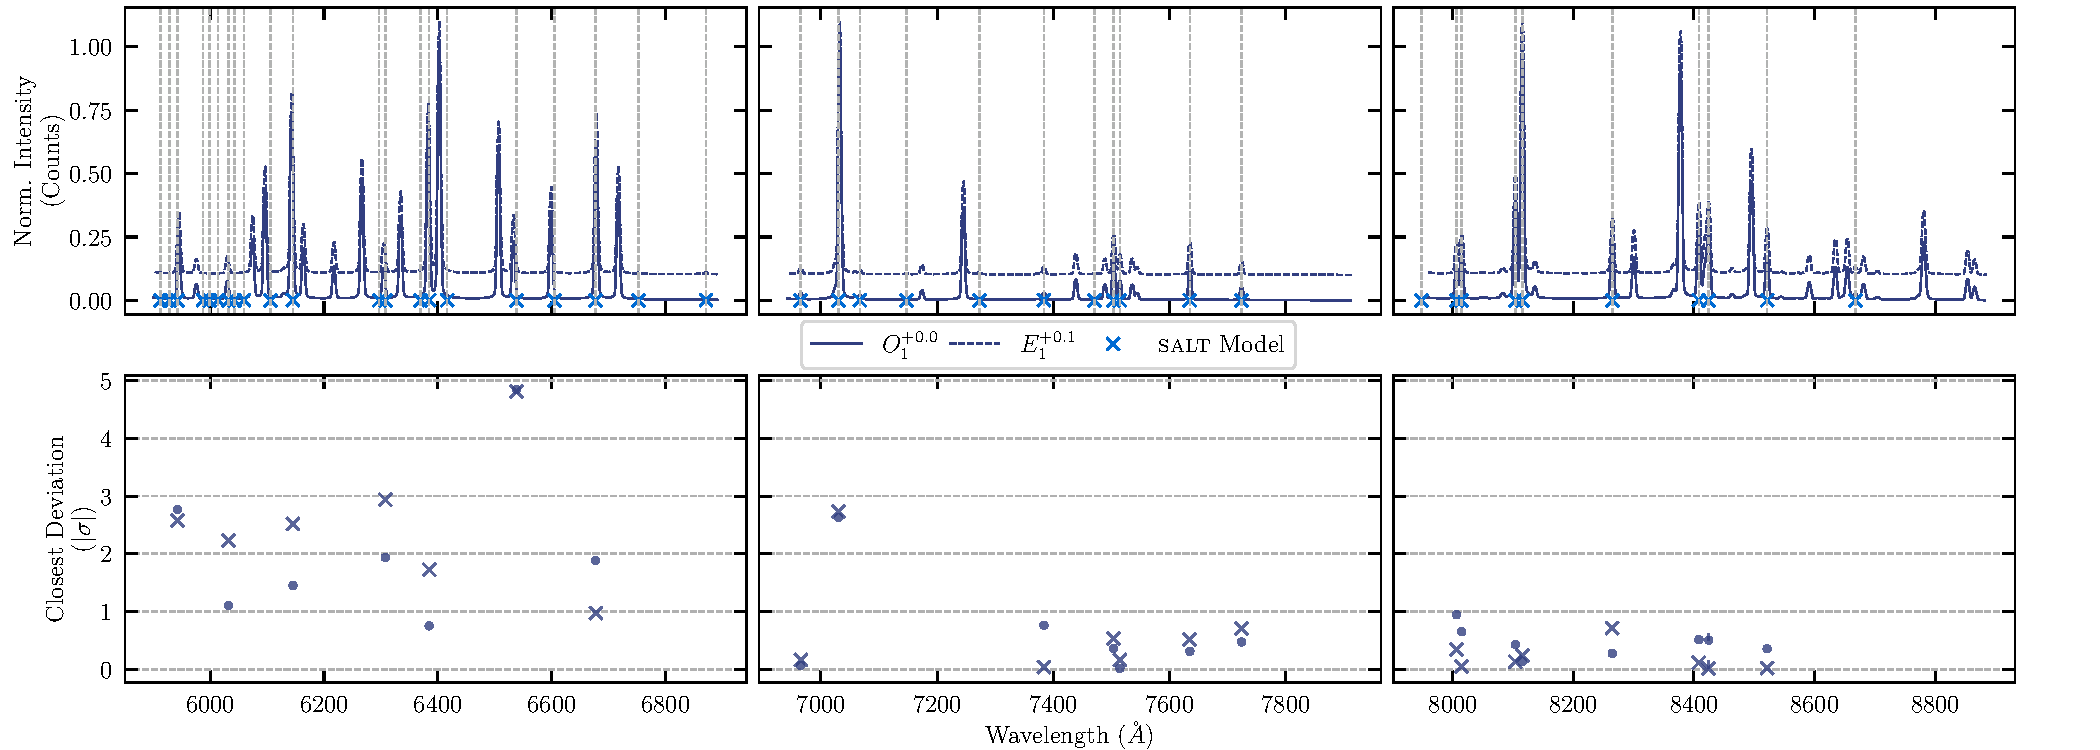
\includegraphics[width = 1.0\textwidth]{3_stops_skylines_arc.pdf}
    \caption{An example of a wavelength solution with a poor fit at shorter wavelengths (bottom left), specifically shown for an arc image. Arc lines are Figure created via the \stops\ \texttt{skyline} method.}
    \label{fig:stops_sky_arc_eg}
\end{figure}
% \begin{figure}
%     \centering
%     \begin{subfigure}[b]{1.0\textwidth}
%         \centering
%         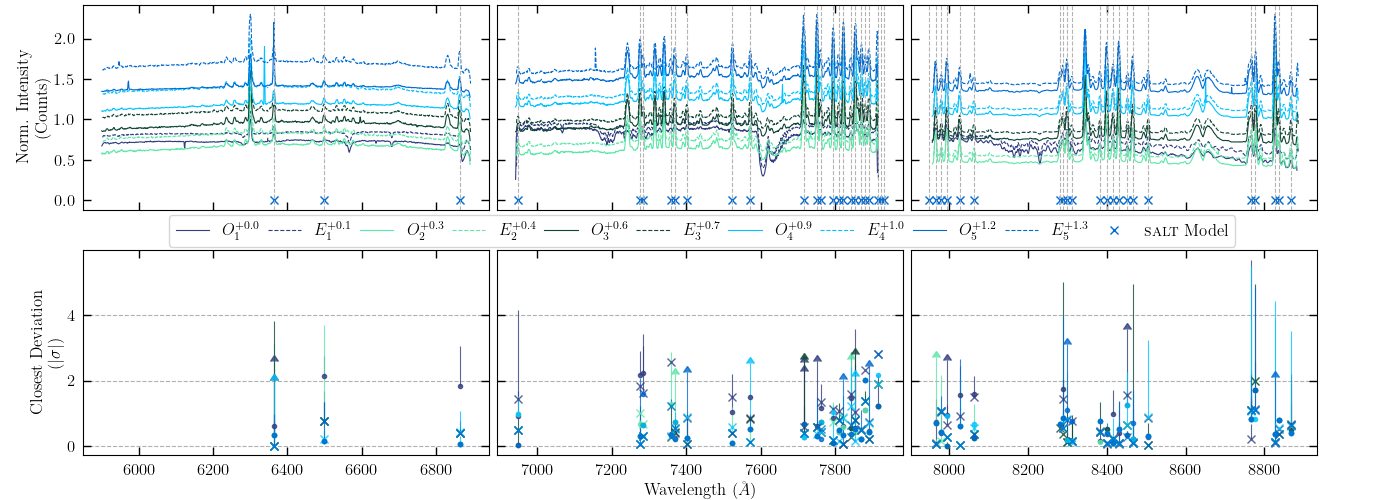
\includegraphics[width=\textwidth]{3_stops_skylines.png}
%         \caption{}
%     \end{subfigure}
%     \vfill
%     \begin{subfigure}[b]{1.0\textwidth}
%         \centering
%         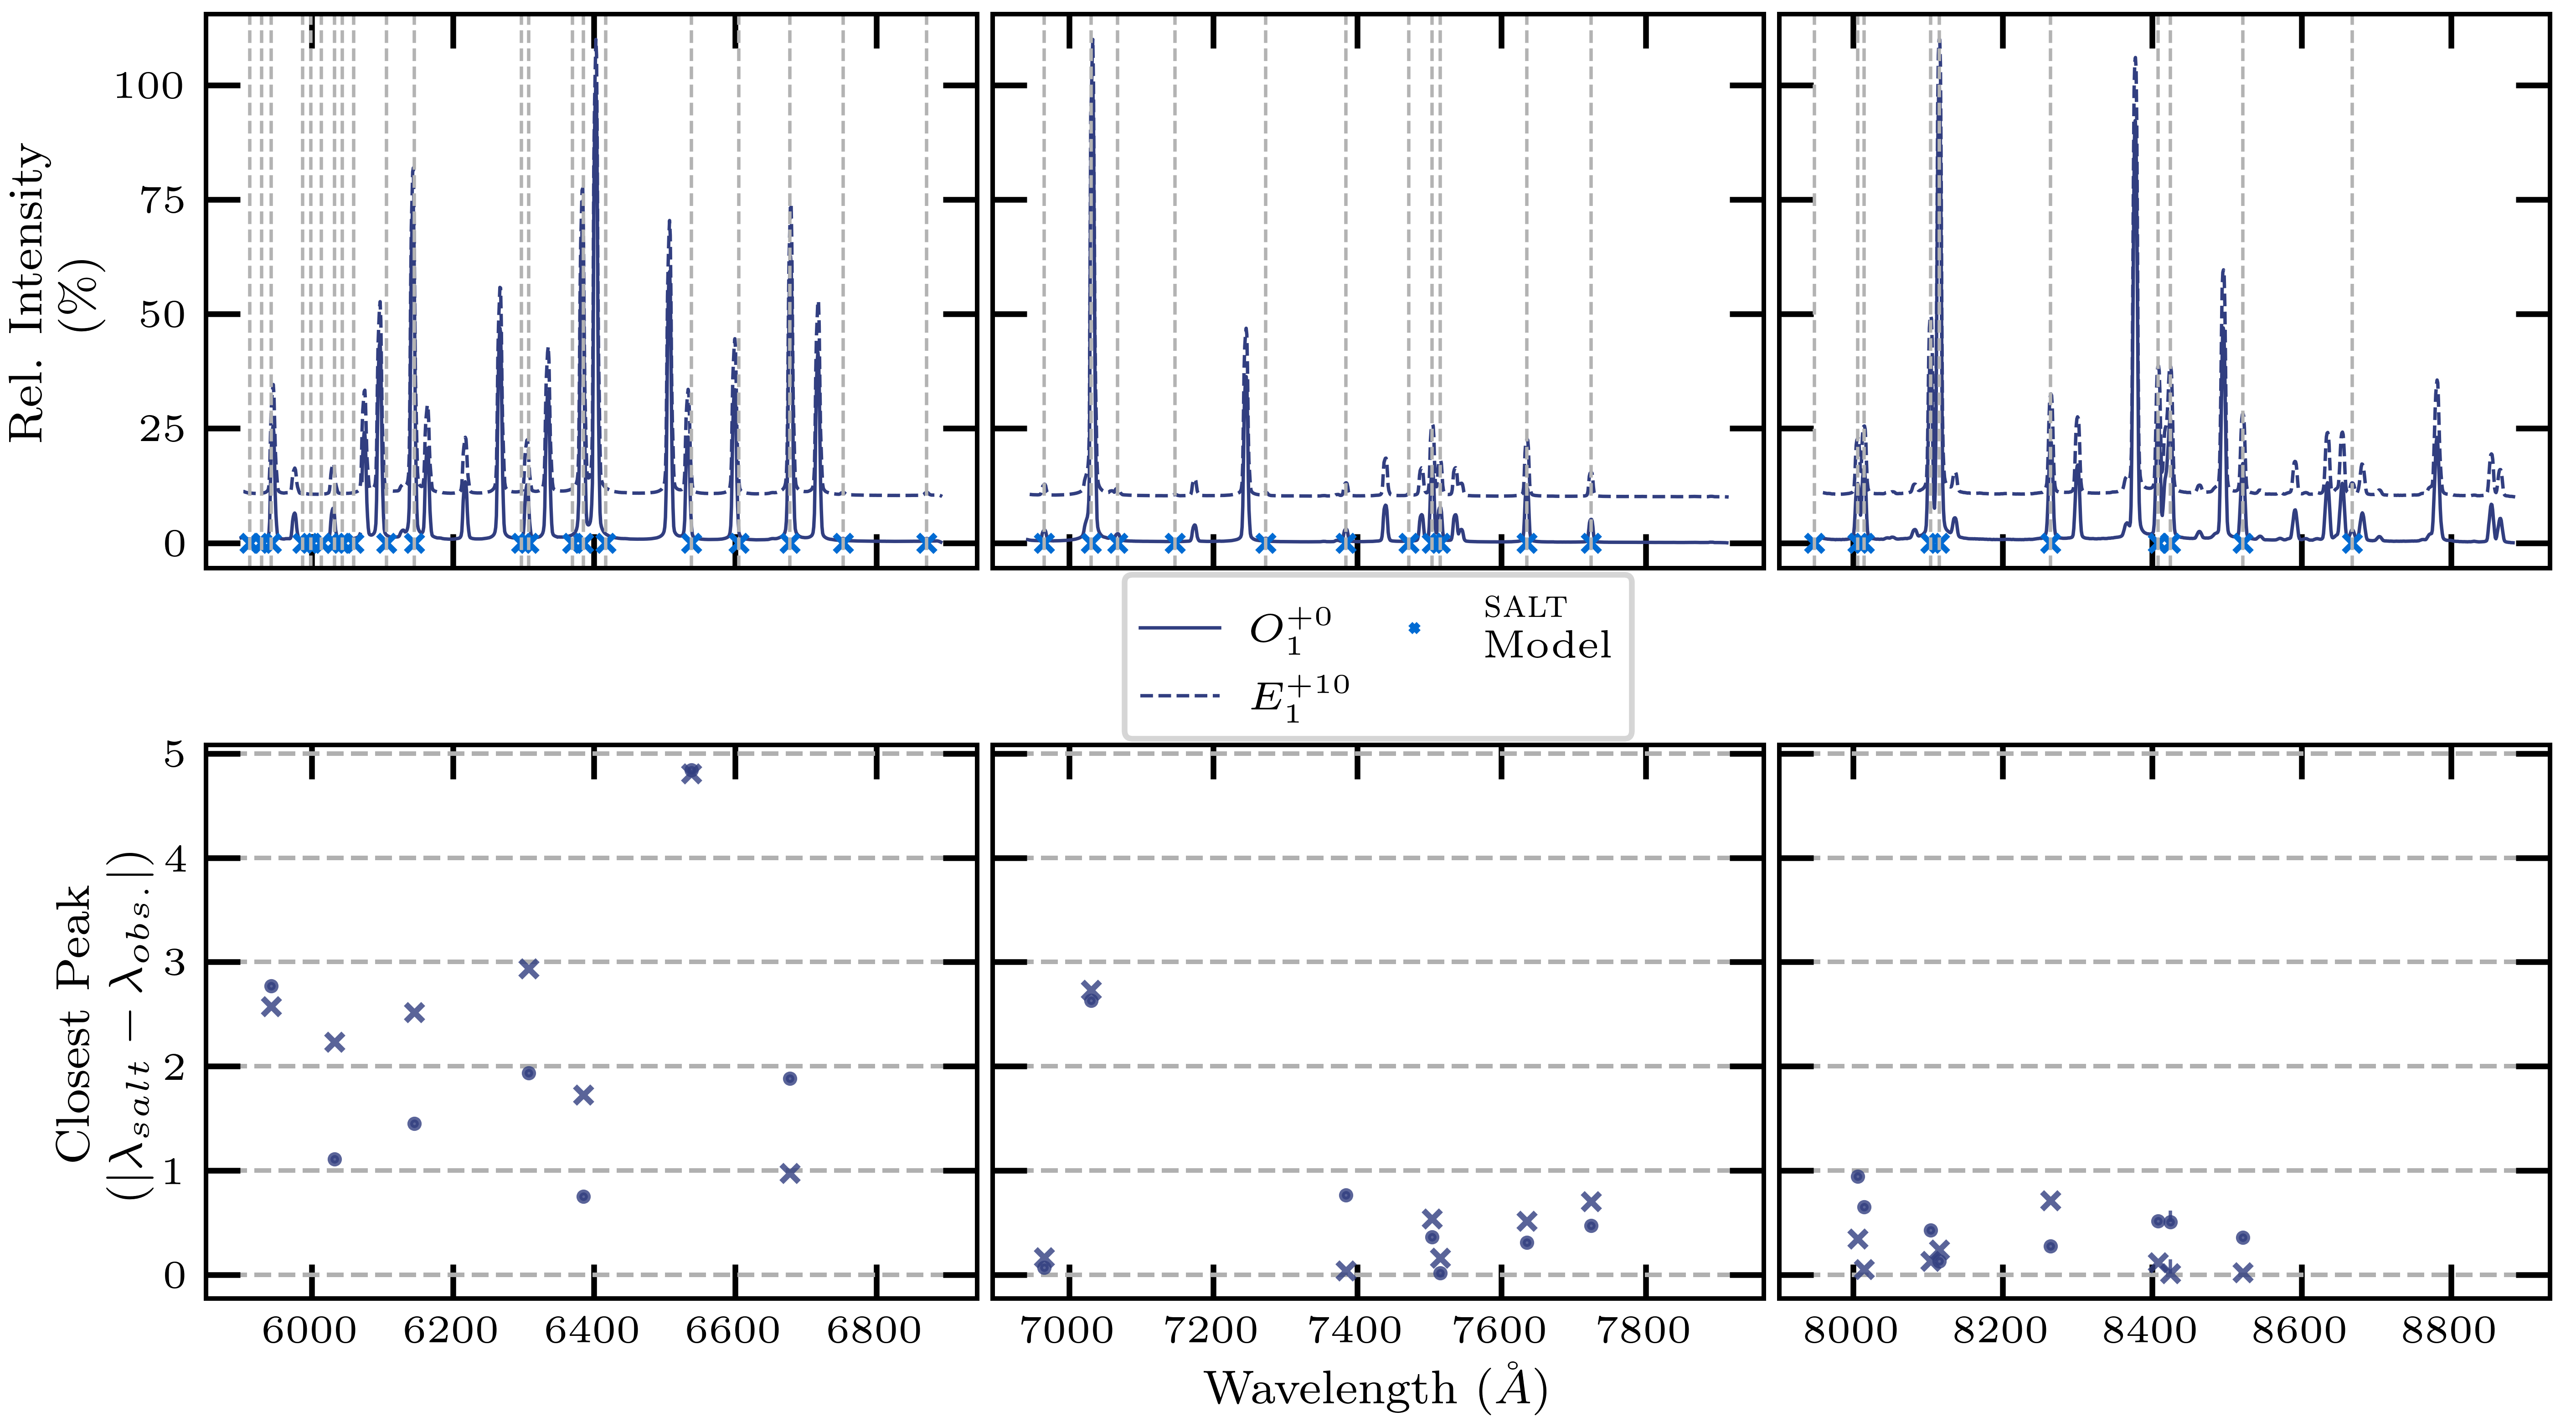
\includegraphics[width=\textwidth]{3_stops_skylines_arc.png}
%         \caption{}
%     \end{subfigure}
%     \caption{The resultant output plot of the \stops\ \texttt{skylines} method. Figure created via the \stops\ \texttt{skyline} method.}
%     \label{fig:stops_sky_eg}
% \end{figure}

% Sky line comparisons allow the user to confirm the accuracy of the wavelength solution across both the rows and columns of the frame. The \texttt{skyline} method naively transforms the wavelength calibrated files, allowing the deviation of a skyline spanning multiple rows to be measured, and compares the observed sky line wavelength positions to those measured by \gls{SALT}, allowing the wavelength deviation of the skylines to be measured.%
The \texttt{skyline} method has been implemented to compare the position of the sky lines on the \gls{SCI} extension, or arc lines in the arc exposure, to the known positions of the sky lines, or arc lines, as measured by \gls{SALT}, respectively.%
\footnote{Both sky and arc lines are available at \url{https://astronomers.salt.ac.za/data/salt-longslit-line-atlas/} .}
This provides an additional check of the accuracy of the wavelength solution across the frame. This method accepts both the \iraf\ \texttt{transform} \gls{FITS} file or the `wmxgbp' \gls{FITS} files created by the \texttt{join} method as the input.

The \texttt{skyline} method loads the wavelength calibrated files, masks the traces present in the frames, transforms the frames from ($x_p$, $y_p$) pixel to (\AA, $y_p$) wavelength units if the frame was not transformed by \texttt{transform},%
\footnote{The transformation applied by the \texttt{skyline} method uses linear interpolation and is thus less accurate at flux conservation than the transformation applied by the \texttt{transform} method.}
and compares the peak wavelength position of the sky lines to the reference sky lines as measured by \gls{SALT}. Finally, a figure is created containing a plot of the background spectra (offset by the respective legend entries superscript) with the known sky lines marked with a vertical line, and a plot of the closest identified peaks of said spectra.

% A spectrum is created after accounting for the \gls{BPM} extension, masking out rows which contain a trace, and transformation, by averaging across the rows of the frames.
% Any inaccuracies of the wavelength solution in the wavelength ($x$, or horizontal) axis are determined by detecting peaks in the spectrum after transformation and comparing their positions to those provided by \gls{SALT}.
Minor variations in the comparison of the sky lines are expected, such as those seen in \autoref{fig:stops_sky_eg}, but any uniform trends, such as those in \autoref{fig:stops_sky_arc_eg} (bottom left), indicate an underlying poor fit across the horizontal axis of the wavelength solution.
% A poor horizontal fit is difficult to spot without supplementary tools.
% 
% Second, any inaccuracies in the wavelength solution in the spatial ($y$, or vertical) axis are determined by comparing the feature widths before and after transformation. Since the sky lines curve slightly across the frame (see \autoref{fig:polsalt_post_wav_cal}), the initial feature widths %relatively straightforward as a perfect wavelength solution will remove any horizontal variation of a sky line spanning multiple rows. The variation may be seen in the transformed frame, as mentioned in \autoref{subsec:iraf_transform}, but is more accurately measured by the \texttt{skyline} method which compares the averaged sky line width before and after transformation. A wavelength solution exhibiting a poor fit across the spatial axis will display broader averaged sky lines than those of a relatively good fit.
The full \stops\ \texttt{skyline} class docstring is given in \autoref{doc:skylines}.

% MARK: Correlate
\subsection{Cross Correlation} \label{subsec:stops_correlate}

\lstinputlisting[
    float,
    language=python,
    style=STOPS_docs,
    caption={The `docstring' for \textbf{cross\_correlate.py}},
    label=doc:corr,
    linerange=corr0-corr1,
    gobble=4,
]{cross_correlate.py}

\begin{figure}[t]
    \centering
    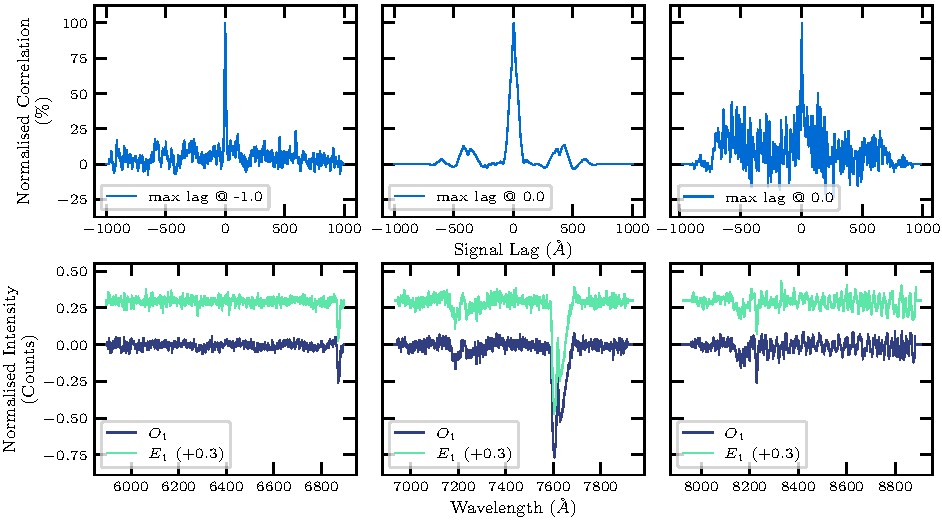
\includegraphics[width = 1.0\textwidth]{3_stops_correlate.pdf}
    \caption{The resultant output plot of the \stops\ \texttt{correlate} method. Figure created via the \stops\ \texttt{correlate} method.}
    \label{fig:stops_corr_eg}
\end{figure}

The \texttt{skyline} method allows for confirmation of a single wavelength solution, but has no means for comparing how the wavelength solutions of two polarization beams differ from each other. As the Stokes results, and thus final polarization results, are determined by the difference between the $O$- and $E$-beams, a direct comparison is not appropriate.

Any observed unpolarized light, however, will reflect equally in both polarization beams and so the general trend of the two spectra may reasonably be expected to follow one another. The \texttt{correlate} method was created to allow for comparisons between the wavelength solutions of the $O$- and $E$-beams of a single exposure or the $O$- or $E$-beams of differing exposures by cross correlating the spectra.

The \texttt{correlate} method loads the \polsalt\ \texttt{spectra extraction} \gls{FITS} files, removes the continuum and separates the \gls{CCD} regions. The relevant \gls{CCD} regions are cross correlated and the correlation peak is plotted and specified in the plot legend, as seen in \autoref{fig:stops_corr_eg}.

Sources under spectropolarimetric observation are generally expected to vary over time and, as such, the ratio of polarized to unpolarized light is also expected to vary. The accuracy of correlation may decrease as features with differences in the polarized component of the polarization beams change, and it is up to the user to determine the validity of the correlation result taking into consideration the two spectra being correlated. The differences in the features of the different spectra are often negligible when compared to the overall continuum of the spectra and are generally only reflected in a change in the intensity of said features when the continuum is removed.
The full \stops\ \texttt{split} class docstring is given in \autoref{doc:corr}.

\pagebreak

% MARK: General Reduction Procedure
\section{General Reduction Procedure}\label{sec:red_proc}

% \begin{figure}[t]
%     \centering
%     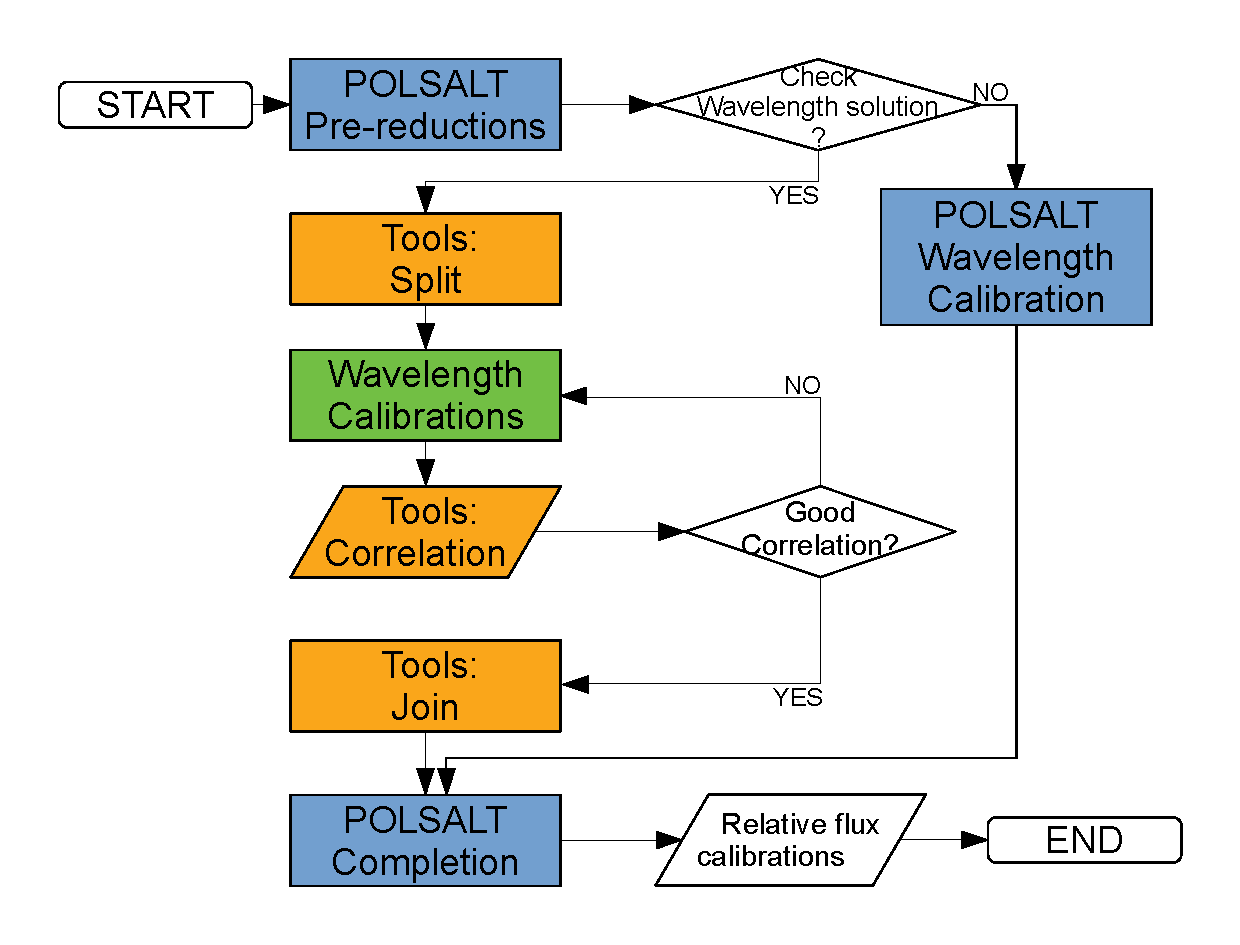
\includegraphics[width = 0.8\textwidth]{3_new_workflow.pdf}
%     \caption{A general workflow for data reductions using a combination of \polsalt, \iraf, and the developed supplementary tools. Diagram adapted from \cite{cooper_HEASA2022}.}
%     \label{fig:new_workflow}
% \end{figure}
% \input{chapter_3/figures/3_reduction_flowchart.tex}
\begin{figure}[t]
    \centering
    \begin{tikzpicture}
        \tikzstyle{ends}    = [rectangle, draw, text centered, minimum height=1.5em, rounded corners]
        \tikzstyle{polsalt} = [rectangle, draw, text centered, minimum height=1.5em, minimum width=6em, fill=cyan]
        \tikzstyle{stops}   = [rectangle, draw, text centered, minimum height=1.5em, minimum width=6em, fill=orange]
        \tikzstyle{iraf}    = [rectangle, draw, text centered, minimum height=1.5em, minimum width=6em, fill=green!50!gray]
        \tikzstyle{choice}  = [diamond,   draw, text centered, text width=5em, aspect=3]
        \tikzstyle{step}    = [rectangle, draw, text centered, minimum height=1.5em]
        \tikzstyle{data}    = [trapezium, draw, text centered, minimum height=1.5em, trapezium left angle=60, trapezium right angle=120]
        \tikzstyle{to}      = [draw, -latex']

        \node (start) [ends] {\hyperref[subsec:reduc_setup]{\textbf{Start}}};

        \node (key_pol) [polsalt, right of=start, xshift=2cm, yshift=1cm] {\textbf{\polsalt}};
        \node (key_stops) [stops, right of=key_pol, xshift=3cm] {\textbf{\stops}};
        \node (key_iraf) [iraf, right of=key_stops, xshift=3cm] {\textbf{\iraf}};

        \node (pol_pre) [polsalt, below of=key_pol] {\hyperref[subsec:pol_raw]{Raw image reduction}};
        \draw [to] (start) -- (pol_pre);
        \node (wav_check) [choice, right of=pol_pre, xshift=3cm, yshift=-1cm] {\polsalt?};
        \draw [to] (pol_pre) -| (wav_check);
        \node (pol_wav) [polsalt, below of=pol_pre, yshift=-1cm] {\hyperref[subsec:pol_wav]{Wavelength calibration}};
        \draw [to] (wav_check) -| node[anchor=south] {Yes} (pol_wav);
        \node (pol_spec) [polsalt, below of=pol_wav, yshift=-3cm] {\hyperref[subsec:pol_spec]{Spectra extraction}};
        \draw [to] (pol_wav) -- (pol_spec);
        \node (pol_rstokes) [polsalt, below of=pol_spec, yshift=-2cm] {\hyperref[subsec:pol_rstokes]{Raw Stokes calculation}};
        \draw [to] (pol_spec) -- (pol_rstokes);
        \node (pol_fstokes) [polsalt, below of=pol_rstokes] {\hyperref[subsec:pol_fstokes]{Final Stokes calculation}};
        \draw [to] (pol_rstokes) -- (pol_fstokes);
        \node (pol_vis) [polsalt, below of=pol_fstokes] {\hyperref[subsec:pol_viz]{Results visualisation}};
        \draw [to] (pol_fstokes) -- (pol_vis);
        \node (stop) [ends, left of=pol_vis, xshift=-2cm] {\textbf{Stop}};
        \draw [to] (pol_vis) -- (stop);

        \node (stops_split) [stops, below of=wav_check, yshift=-1cm] {\hyperref[subsec:stops_split]{\texttt{split}}};
        \draw [to] (wav_check) -- node[anchor=west] {No} (stops_split);
        \node (iraf_id) [iraf, right of=stops_split, xshift=3cm] {\hyperref[subsec:iraf_identify]{\texttt{identify}}};
        \draw [to] (stops_split) -- (iraf_id);
        \node (iraf_reid) [iraf, below of=iraf_id] {\hyperref[subsec:iraf_reidentify]{\texttt{reidentify}}};
        \draw [to] (iraf_id) -- (iraf_reid);
        \node (iraf_fit) [iraf, below of=iraf_reid] {\hyperref[subsec:iraf_fitcoords]{\texttt{fitcoords}}};
        \draw [to] (iraf_reid) -- (iraf_fit);

        \node (stops_join) [stops, left of=iraf_fit, xshift=-3cm] {\hyperref[subsec:stops_join]{\texttt{join}}};
        \draw [to] (iraf_fit) -- (stops_join);
        
        % Make optional node
        \node (iraf_trans)  [iraf, below of=iraf_fit] {\hyperref[subsec:iraf_transform]{\texttt{transform}}};
        % Make optional path
        \draw [to] (iraf_fit) -- (iraf_trans);
        
        \node (stops_sky)   [stops, left of=iraf_trans, xshift=-3cm, yshift=-1cm] {\hyperref[subsec:stops_skyline]{\texttt{skyline}}};
        \draw [to] (stops_join) -- (stops_sky);
        % Make optional path
        \draw [to] (iraf_trans) -| (stops_sky);
        
        \node (stops_corr)  [stops, right of=pol_spec, xshift=3cm, yshift=-2cm] {\hyperref[subsec:stops_correlate]{\texttt{correlate}}};
        \draw [to] (stops_join) -| (pol_spec.east) |- (stops_corr);
        
        \node (corr_check)  [choice, below of=iraf_trans, yshift=-1cm] {Good~$f_\lambda(x, y)$?};
        \draw [to] (stops_sky) -| (corr_check);
        \draw [to] (stops_corr) -- (corr_check);
        \draw [to] (corr_check) |- node[anchor=west] {Yes} (pol_rstokes);
        \draw [to] (corr_check) -| node[anchor=north] {No} ++(2.5cm, 5cm) -- (iraf_id);

    \end{tikzpicture}
    \caption{A general workflow for data reductions using a combination of \polsalt, \iraf, and \stops. Diagram adapted from \cite{cooper_HEASA2022}.}
    \label{fig:new_workflow}
\end{figure}

This section aims to provide a comprehensive discussion of the modified reduction procedure, an example of which is provided in \autoref{app:reduction}. As users all employ a variety of operating systems, language environments, and software setups, not much emphasis will be placed on how to get the software running or the managing of files; instead, the general order, seen in \autoref{fig:new_workflow}, and commands necessary to complete each step of the reduction process are discussed, assuming that the software is running as intended.

\subsection{Initial Setup} \label{subsec:reduc_setup}

It is important to note that while \polsalt\ was developed in Python~$2$ ($2.7$), the \stops\ supplementary tools were developed in, and require, Python~$3$ ($3.11+$), as well as the other requirements mentioned in \autoref{sec:stops}. While managing multiple versions of Python introduces some extra complication, it would not have been reasonable to develop \stops\ in Python~$2$, as it has been deprecated, nor would it have been reasonable to update \polsalt\ to Python~$3$.

It is therefore recommended that the different versions of Python are managed using separate virtual environments. While the \texttt{anaconda} package manager was used in this study and is recommended, any package manager may be used. The \texttt{anaconda} environments are aliased `\textbf{salt}' for Python $2.7$ and `\textbf{stops}' for Python $3.11$. When Listings are provided (see for example \autoref{code:polsalt_launch} or the Listings in \autoref{subsec:reduc_pre} below), the \texttt{anaconda} environment is activated at the start of the Listing, otherwise it is assumed the previously specified environment is still active.

\pagebreak

It is recommended to use \polsalt\ through the \gls{GUI} as it provides a user-friendly environment while also sequentially listing each step of the reduction process in a dropdown menu, as seen in \autoref{fig:polsalt_gui}. Reductions are possible, however, purely through the \gls{CLI} using the \polsalt\ `beta' scripts.

% MARK: Pre-reductions
\subsection{\textsc{polsalt} Pre-Reductions} \label{subsec:reduc_pre}

\begin{figure}[t]
    \centering
    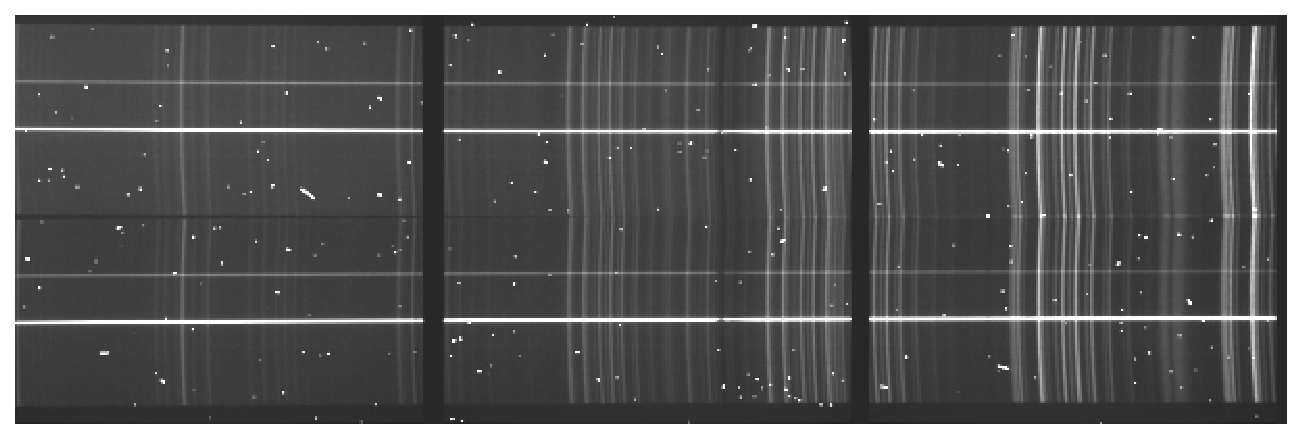
\includegraphics[width = 1.0\textwidth]{3_pre_wav_cal.pdf}
    \caption{The \gls{SCI} extension of a typical spectropolarimetric \acs{FITS} file taken with the \gls{SALT} \gls{RSS}, after basic \polsalt\ \gls{CCD} reductions have been completed. Figure created from the \stops\ \texttt{split} output.}
    \label{fig:polsalt_pre_wav_cal}
\end{figure}

The \polsalt\ reduction process requires a file structure such that the raw data received from \gls{SALT} is located in a folder named using the observing date with a sub-folder named raw, following the format \texttt{YYYYMMDD/raw/}. This directory structure allows \polsalt\ to create a `working' directory following the format \texttt{YYYYMMDD/sci/} which contains all the files modified during the reduction process. Multiple reduction procedures using the same data may therefore be separated by simply renaming the \texttt{sci/} sub-folder.

The \polsalt\ \gls{GUI} may be launched by opening a \gls{CLI} and running the commands given in \autoref{code:polsalt_launch}. Once the window, depicted in \autoref{fig:polsalt_gui}, has launched, ensure that the first two paths at the top of the window point to the \polsalt\ and working directories, as seen in \autoref{fig:polsalt_gui}. The `raw image reduction' entry may then be selected from the dropdown menu and the pre-reductions run.

Alternatively, if the data already includes `mxgbp' \gls{FITS} files in the \texttt{YYYYMMDD/sci/} working directory, a \gls{CLI} may be used to complete the initial pre-reductions using
\begin{lstlisting}[language=bash]
$ cd (*@<\textit{OBSDATE}>@*)/sci
$ conda activate salt
$ python ~/polsalt/scripts/reducepoldata_sc.py (*@<\textit{OBSDATE}>@*)
\end{lstlisting}
{\parskip=0pt which} will start the full \polsalt\ reduction process. This process is quit once the \polsalt\ \texttt{wavelength calibration} \gls{GUI} opens, and the alternate wavelength calibration procedure is followed.

\pagebreak

% MARK: Wavelength Calibration
\subsection{Wavelength Calibration} \label{subsec:reduc_wav}

The wavelength calibrations may now be completed in \iraf. This section concerns the procedure for parsing the \gls{FITS} files to and from both \iraf\ and \polsalt, as well as the relevant task names and methods to be run to complete the calibrations. A base working case of each of the tasks and methods are presented in \autoref{code:stops_split} to \ref{code:stops_join}, but it should be noted that the art of wavelength calibration consists of modifying the parameters to achieve a well-fit calibration function.% This process depends heavily, and varies greatly, based on the user and as such not all use cases can be discussed.

% MARK: Prep for IRAF
\subsubsection{Preparing the Data for \iraf}

Splitting the data is presented in \autoref{code:stops_split}. The \stops\ \texttt{split} method may take multiple parameters, as seen in \autoref{sec:stops}, but default parameters should be used wherever possible. The most notable parameters are the directory, which defaults to the current working directory of the \gls{CLI}, the split row, which defaults to \polsalt's default center row, and the save prefix, which defaults to `\texttt{obeam}' and `\texttt{ebeam}'.
% As an aside, the save prefix may be worth changing as, later in the reduction process, the \polsalt\ raw Stokes reductions indiscriminately selects files named \texttt{YYYYMMDD/sci/e*.fits}, which would include the split `wmxgbp' \gls{FITS} files (ebeam*.fits). This naming conflict is revisited and addressed later on in the reduction process and is thus not of any concern.

% MARK: IRAF wavelength calibrations
\subsubsection{\iraf\ Wavelength Calibrations}

The \iraf\ wavelength calibrations are performed using the tasks described in \autoref{sec:iraf}, namely the \texttt{identify}, \texttt{reidentify}, \texttt{fitcoords}, and optionally \texttt{transform} tasks.

{\noindent In} general, these tasks are run directly in the \iraf\ terminal using:%
\footnote{Please see the \iraf\ help docs, available at \url{https://astro.uni-bonn.de/~sysstw/lfa_html/iraf/iraf.html}, on the relevant tasks for a comprehensive discussion of the parameters available.}

\begin{lstlisting}[language=bash]
cl> identify arc_files
cl> reidentify arc_ref arc_files
cl> fitcoords arc_files fit_2d
cl> transform files tr_file fit_2d
\end{lstlisting}
{\parskip=0pt where} `arc\_files' refers to a list or file containing the \gls{FITS} files relevant to the task, `arc\_ref' refers to the \gls{FITS} file previously identified, `fit\_2d' refers to the name to be used for the final two-dimensional wavelength solution, and `tr\_file' refers to the new name for the transformed input `files'.

The interactive tasks take up the bulk of the reduction time as this is where the fine-tuning of the reduction is done, through the use of cursor (or colon) commands, which allow modification of the parameters mid-reduction. Task parameters may, however, be edited beforehand within the \iraf\ terminal using the \texttt{eparam} task, and optionally saved, and quit or run using a combination of \texttt{:w}, and \texttt{:q} or \texttt{:go} cursor commands, respectively.

The reduction process in \autoref{app:reduction}, namely \autoref{code:iraf_id} to \ref{code:iraf_transform}, describes how the tasks may be scripted and saved for posterity. It is recommended to create an \iraf\ Command Language (cl) script for each task to keep track of which parameters were used and for simple recalibrations. The scripts are created using the \texttt{mkscript} task which interactively asks for a task to script and parameters to use. Multiple tasks may be appended to an \iraf\ script, allowing for the parameters of both beams to be tracked.

Running an \iraf\ script may be done by running:
\begin{lstlisting}[language=bash]
cl> cl < script_name.cl
\end{lstlisting}
{\parskip=0pt but} is not suggested for interactive scripts, which run best when simply copied from the \texttt{<.../>sci/script\_name.cl} file to the \iraf\ terminal.

\pagebreak

% MARK: Post IRAF
\subsubsection{Preparing the Data for \polsalt}

After the wavelength calibrations have been completed, the wavelength solution is parsed back into the format expected by \polsalt. Joining the separate beams with their respective wavelength solutions is performed in the \gls{CLI} following \autoref{code:stops_join}.

Similar to the \texttt{split} procedure, the \texttt{join} procedure has the same defaults defined. The onus of keeping track of any previously changed default parameters falls to the user, but logging is implemented in \stops\ (see the discussion on help documentation in \autoref{sec:stops}) which allows for later reference of any changed parameters.

% MARK: Skyline checks
\subsubsection{Sky Line Checks} \label{subsec:reduc_sky}

The optional \iraf\ \texttt{transform} task and \stops\ \texttt{skylines} method are used to confirm the wavelength solution across the frame (see \autoref{subsec:stops_skyline}) by transforming and comparing known and observed sky line wavelength positions, respectively.

The \texttt{skyline} method is run in the \gls{CLI} following \autoref{code:stops_sky}. As with the rest of \stops, default parameters describe the overplotting behavior for the $O$- and $E$-beams, the skylines provided by \gls{SALT}, and the calculated variation of the wavelength axis of a frame.

\subsubsection{Cross Correlation Checks} \label{subsec:reduc_corr}

The \texttt{correlate} method is run in the \gls{CLI} following \autoref{code:stops_corr}. The input of the \texttt{correlate} method takes the output of the \polsalt\ \texttt{spectra extraction} and is thus only run thereafter, but is mentioned here as the completion of the \polsalt\ reductions is not discussed in much depth. If the user wishes to compare the $O$- and $E$-beams of a single file then only that image name is to be provided, otherwise it is assumed that the user wishes to compare the same polarization beam across each file provided.

\subsubsection{Cleaning Up the \iraf\ and \stops\ Output}

Before the final \polsalt\ reductions, it is recommended that the user `clean up' the \texttt{sci/} directory of all \iraf\ and \stops\ files since the `wmxgbp' \gls{FITS} files are all that is expected by \polsalt. The \polsalt\ methods use wildcard file collection and as such any errant detections of files added by the user will result in unexpected crashes. It is suggested to move any additional files to a new subfolder following \autoref{code:gen_clean}, but they may also be removed using:
\begin{lstlisting}[language=bash]
$ rm beam*.fits arc*.fits frame* <any user created files>
\end{lstlisting}

% MARK: Complete reductions
\subsection{\textsc{polsalt} Reduction Completion} \label{subsec:reduc_com}

Reductions may now be completed using \polsalt. The reduction process consists of correcting for the wollaston tilt, extracting the spectra, creating the Stokes files, and displaying the results. The `beta' version of \polsalt\ provides access to a \gls{GUI} but may also be handled entirely through a \gls{CLI} as scripts.

% MARK: POLSALT GUI
\subsubsection{\polsalt\ Beta in the \gls{GUI}}

The reduction process using the \polsalt\ \gls{GUI} is completed by selecting and, when applicable, interactively modifying the reduction step through the interactive windows, one-by-one, from the \gls{GUI}'s dropdown menu, as explained in \autoref{app:reduction} (\autopageref{code:stops_corr} onwards).%
\footnote{See the official \href{https://github.com/saltastro/polsalt/wiki}{\polsalt\ wiki} or alternative online resources such as the \href{https://saltworkshop2022.salt.ac.za/wp-content/uploads/2022/11/DG_polsalt_SALT_workshop_2022_finalversion.pdf}{\gls{SALT} workshop slides}.}

% Covering the \gls{CLI} implementation first, the wavelength solution needs to be applied to all the \gls{FITS} files and the tilt introduced by the wollaston prism must be corrected for. This is done through the command:
% \begin{lstlisting}[language=bash]
% $ python ~/polsalt/scripts/correct_files.py w*fits
% \end{lstlisting}
% {\parskip=0pt where} the `w*.fits' is a wildcard expression that lists the \gls{FITS} files that have a \gls{WAV} extension and returns it to the \polsalt\ script.

% Next, the spectra in each \gls{FITS} file are extracted using the command:
% \begin{lstlisting}[language=bash]
% $ python ~/polsalt/scripts/pol_extract.py c*.fits \
% > --yo A --ye B --dy C
% \end{lstlisting}
% {\parskip=0pt where} the center row of the spectra for the $O$- and $E$-beams, \texttt{A} and \texttt{B}, as well as the spectral width, \texttt{C}, are compulsory integer values. These may be found through \gls{FITS} viewing software such as ds9%
% \footnote{Available at \protect\url{https://sites.google.com/cfa.harvard.edu/saoimageds9}} or more manually through python.

% The Stokes files may then be calculated and created using the command:
% \begin{lstlisting}[language=bash]
% $ python ~/polsalt/scripts/pol_stokes.py
% \end{lstlisting}
% {\parskip=0pt which} automatically detects the \gls{FITS} files using the wildcards `e*fits' for raw Stokes and `*\_h*.fits' for the final Stokes calculations. The deletion of the \gls{FITS} files created in the supplementary \texttt{split} method may be deleted in the \texttt{join} method specifically to avoid this naming convention clash, but may also be avoided by providing an alternate default subscript to the supplementary methods.

% Finally, the results of the Stokes calculations may be viewed using the command:
% \begin{lstlisting}[language=bash]
% $ python polsalt/specpolview.py *_stokes.fits
% \end{lstlisting}
% {\parskip=0pt where} a file name, which may also use a wildcard, is provided as well as optional para\-meters to define the binning (\texttt{bin=[int]A} where [int] refers to an actual integer value), error bars (\texttt{errors=True|False}), choice of plot (\texttt{type=Ipt|Iqu} for unbinned intensity and either polarization percentage and polarization angle, or $Q$ and $U$ Stokes parameters), save options (\texttt{save=[text][plot] where either or both `text' and `plot' may be provided}), and a debug mode (\texttt{debug=False|True}).

% MARK: POLSALT CLI
\subsubsection{\polsalt\ Beta through a \gls{CLI}}

Both \gls{GUI} and \gls{CLI} implementations of the \polsalt\ beta pipeline access the same script files. Although the \gls{GUI} is more user-friendly, the \gls{CLI} offers a more streamlined approach to the reduction process, allowing the reduction process to be automated once the \iraf\ wavelength solution is known and parsed into the `wmxgbp' \gls{FITS} file format. A modified version of the \polsalt\ beta \texttt{reducepoldata\_sc.py} script (see \autoref{code:pol_reduc}) is used to run the entire reduction process without needing to select which process to run next, using:
\begin{lstlisting}[language=bash]
$ python reducepoldata_sc.py YYYYMMDD
\end{lstlisting}
{\parskip=0pt where} the only modification made to the \texttt{reducepoldata\_sc.py} script file is the removal of a call to the \texttt{specpolwavmap} method.
% The \texttt{imred} and \texttt{specpolwavmap} function calls before \texttt{specpolextract\_sc} should be commented out, since the raw images have already been processed and the wavelength calibrations were completed using \stops\ and \iraf.

\newcommand*{\Comment}[1]{\hfill\makebox[7.0cm][l]{#1}}%
\begin{lstlisting}[
    float,
    language=Python,
    style=IRAF_DB,
    caption={The modified \texttt{reducepoldata\_sc.py} script file.},
    label=code:pol_reduc]
import os, sys, glob, shutil
poldir = '/home/justin/polsalt-beta/'(*@\Comment{\# Will differ according to user}@*)

reddir=poldir+'polsalt/'
scrdir=poldir+'scripts/'
sys.path.extend((reddir,scrdir,poldir))

datadir = reddir+'data/'
import numpy as np
from astropy.io import fits as pyfits
from specpolview import printstokes
from imred import imred
from specpolwavmap import specpolwavmap
from specpolextract_sc import specpolextract_sc
from specpolrawstokes import specpolrawstokes
from specpolfinalstokes import specpolfinalstokes

print sys.argv
obsdate = sys.argv[1]
print obsdate
os.chdir(obsdate)
if not os.path.isdir('sci'): os.mkdir('sci')
shutil.copy(scrdir+'script.py','sci')
os.chdir('sci')

#basic image reductions
infilelist = sorted(glob.glob('../raw/P*fits'))
imred(infilelist, './', datadir+'bpm_rss_11.fits', crthresh=False, cleanup=True)

#basic polarimetric reductions
logfile='specpol'+obsdate+'.log'

(*@\Comment{\# The following lines may be removed or commented out as below}@*)
# #wavelength map
# infilelist = sorted(glob.glob('m*fits'))
# linelistlib=""
# specpolwavmap(infilelist, linelistlib=linelistlib, logfile=logfile)

#background subtraction and extraction
infilelist = sorted(glob.glob('wm*fits'))
extract = 10.   # star +/-5, bkg= +/-(25-35)arcsec:  2nd order is 9-20 arcsec away
locate = (-120.,120.)    # science target is brightest target in whole slit
#locate = (-20.,20.)

specpolextract_sc(infilelist,logfile=logfile,locate=locate,extract=extract)
#specpolextract_sc(infilelist,logfile=logfile,locate=locate,extract=extract,docomp=True,useoldc=True)

#raw stokes
infilelist = sorted(glob.glob('e*fits'))
specpolrawstokes(infilelist, logfile=logfile)

#final stokes
infilelist = sorted(glob.glob('*_h*.fits'))
specpolfinalstokes(infilelist, logfile=logfile)

\end{lstlisting}

The \polsalt\ beta \texttt{reducepoldata\_sc.py} copies a \texttt{script.py} file into the science working directory, `YYYYMMDD/sci/', which provides analysis scripts for analysis and modification of the \polsalt\ beta results. These tools consist of data culling for the final Stokes calculations, text and plot output, relative flux calibration corrections, and synthetic filtering of polarization results.

The \polsalt\ analysis scripts may be run using:
\begin{lstlisting}[language=bash]
$ python script.py
\end{lstlisting}
{\parskip=0pt followed} by \texttt{specpolfinalstokes.py}, \texttt{specpolview.py}, \texttt{specpolflux.py}, or \texttt{specpol\-filter.py}, for the different analysis modes, respectively.%
\footnote{Please see \url{https://github.com/saltastro/polsalt/wiki/Linear-Polarization-Reduction.--Beta-version} for a comprehensive discussion of the \polsalt\ beta analysis scripts.}
